\documentclass[a4paper,12pt]{report}

\usepackage{alltt, fancyvrb, url}
\usepackage{graphicx}
\usepackage[utf8]{inputenc}
\usepackage{float}
\usepackage{longtable}
\usepackage{hyperref}
\usepackage{array}

% Questo commentalo se vuoi scrivere in inglese.
\usepackage[italian]{babel}
\usepackage[italian]{cleveref}

\title{Resplan \\ \large Record, edit \& plan}

\author{Alessandro Antonini, Gabriele Menghi, Luca Pasini, Giacomo Sirri}
\date{\today}


\begin{document}

\maketitle

\tableofcontents

\chapter{Analisi}

Resplan modella una Digital Audio Workstation (DAW) specifica per contenuti vocali, quali podcast, audiolibri e audiolezioni.
L’applicazione si propone di fornire un ambiente semplice ed intuitivo nel quale l’utente potrà pianificare, registrare ed editare in tracce separate vari file audio.

Sebbene sul mercato esistano altri applicativi che svolgono parte di queste funzioni, la caratteristica che contraddistingue Resplan è l’intenzione di guidare sia l’utente professionale che quello inesperto al corretto utilizzo degli strumenti forniti. Il software infatti preimposterà i vari parametri e organizzerà il progetto nel modo più opportuno. Inoltre Resplan supporterà l’utente anche nella fase di pianificazione e stesura del contenuto da realizzare, ovvero in tutto quel processo preliminare alla registrazione ed editing del contenuto stesso.


\section{Requisiti}

Come descritto nell’analisi, in una prima fase, l’applicazione supporterà l’utente nella pianificazione del contenuto da realizzare, organizzando il progetto in tracce separate per ogni persona o tipologia di sorgente audio.

Sarà possibile dividere la timeline in sezioni e poi creare per ogni canale delle clip vuote corrispondenti alle varie parti audio da realizzare.
Le parti potranno essere riempite importando nell’applicazione file preesistenti, oppure direttamente all’interno di Resplan acquisendo da un'interfaccia audio collegata al sistema.

I contenuti potranno poi essere tagliati, spostati e processati.
Infine l’applicazione provvederà a sommare tutte le tracce in un’unica traccia stereo, la quale potrà essere esportata dall’applicazione in formato audio WAVE.
Di seguito sono riportati i requisiti in forma compatta e suddivisi per tipologia.

\subsubsection{Requisiti funzionali}
\begin{itemize}
	\item Pianificazione
	\begin{itemize}
	    \item Creazione di tracce corrispondenti a speakers, file audio, effetti sonori. 
	    \item Suddivisione della timeline in sezioni.
        \item Posizionamento nella timeline delle parti da inserire o registrare per ogni traccia.
        \item Possibilità di associare testi ad ogni parte da registrare.
	\end{itemize}
	\item Produzione
	\begin{itemize}
	    \item Registrazione: All’utente viene fornita la possibilità di registrare su uno o più canali, corrispondenti agli oratori. I canali vengono sommati nel canale master.
	    \item Integrazione con tracce audio preesistenti: L’utente può importare file audio esterni all’interno del progetto.
	\end{itemize}
	\item Editing
	\begin{itemize}
	    \item Spostare nella timeline di progetto le varie clip audio.
        \item Tagliare l’audio acquisito. 
        \item Mixing, cioè possibilità di modificare volume, panning, equalizzazione e dinamica delle tracce audio.
	\end{itemize}
	\item Preview
	\begin{itemize}
	    \item Possibilità di ascoltare l’audio del progetto in tempo reale prima dell’esportazione.
	\end{itemize}
	\item Finalizzazione
	\begin{itemize}
	    \item Mastering: equalizzazione, dinamica (compressione e limiting), riverbero.
	    \item Esportazione del canale master in un file audio in formato WAVE stereo (.wav).
	\end{itemize}
	\item Controllo dell’applicazione
	\begin{itemize}
	    \item Salvataggio dei file di progetto: per ogni progetto vengono memorizzati i parametri di ogni traccia audio e le clip audio presenti con relativa posizione nella timeline.
	    \item Apertura dei file di progetto esistenti: l’applicazione permette di aprire un progetto per volta.
	    \item Possibilità di settare un progetto come “template”: quando l’utente desidera creare un nuovo progetto, l’applicazione, invece di aprire un progetto vuoto, apre il template.
	\end{itemize}
\end{itemize}

\subsubsection{Requisiti non funzionali}
\begin{itemize}
    \item L’applicazione prevede una grafica interattiva, con la possibilità di fare il Drag & Drop per spostare e ridimensionare le clip.
\end{itemize}

\section{Analisi e modello del dominio}
Ogni singolo suono generato nel mondo è diverso e unico. Spesso non ci si rende conto di quanto nella vita di tutti i giorni sia estremamente importante poter catturare una vibrazione sospesa nell’aria, ovvero l’audio, e riprodurlo. Questa pratica rende possibili molte nostre abitudini come ascoltare una canzone su Spotify, guardare un tutorial su Youtube, ascoltare un audiolibro, mandare un audio su WhatsApp, conversare con un assistente virtuale o ascoltare un podcast.
Forse proprio per questo l’evoluzione delle tecniche e degli strumenti a disposizione per la creazione di contenuti audio è stata estremamente veloce e tuttora continua inarrestabile.

Moltissime tecnologie sono state protagoniste di questo sviluppo, ma uno dei passaggi chiave è stato quello dal dominio analogico a quello digitale, che è stato permesso grazie all’invenzione e all’evoluzione dei calcolatori. 
Resplan è una Digital Audio Workstation, ovvero un software che permette di registrare ed editare l’audio in digitale. Si rendono pertanto necessari per la comprensione delle scelte progettuali una breve descrizione del dominio e alcuni cenni storici sullo sviluppo delle tecnologie audio.

Prima che venissero adottate le Digital Audio Workstation, la registrazione in studio avveniva per mezzo di hardware analogici come mixers, registratori, processori di segnale.
Gli artisti svolgevano la loro performance e registravano le varie parti (voce, chitarra, batteria, basso, ecc…) in tracce separate con l’ausilio di registratori a nastro multitraccia.
Ogni traccia audio registrata poteva essere riprodotta e inviata ad un canale del mixer, dove veniva processata individualmente ed eventualmente inviata a processori esterni (come equalizzatori, compressori, saturatori, ecc…).
Il mixer sommava tutte le tracce in un unico canale master, che veniva poi registrato in una unica traccia stereo per essere finalizzato, stampato sui vari supporti audio e distribuito nei punti vendita.
La digitalizzazione di questo processo ha permesso di abbattere alcuni vincoli che la registrazione analogica imponeva, permettendo una maggior flessibilità e libertà nell’incisione dei prodotti audio, oltre che la riduzione dei costi dovuti all’attrezzatura hardware.
Una delle facilitazioni che le D.A.W. forniscono è quella di poter traslare nel tempo parti di un'unica registrazione, che potrà quindi essere tagliata, scomposta e riarrangiata nella timeline a piacimento. Questo è stato possibile introducendo il concetto di “clip” audio, che rappresenta un segmento di audio indipendente. 
Un altro vantaggio di lavorare con l’audio in digitale è quello di poter cambiare progetto rapidamente. Infatti lavorando in analogico è necessario effettuare il cosiddetto “recall”, ovvero il ripristino a mano della posizione di tutti i knob e fader dei dispositivi analogici utilizzati. Operazione che può richiedere ore di lavoro.

Ovviamente nel passaggio da analogico a digitale si è dovuto far fronte a varie limitazioni o problematiche come quella della rappresentazione di un segnale analogico continuo (quindi composto da infiniti valori) in un dominio digitale che memorizza solo valori finiti. Viene introdotto il sampling audio, pratica che permette la conversione di audio analogico in digitale tramite il campionamento del segnale originale, seguito da una quantizzazione dei valori campionati in ogni istante.
Il segnale audio in digitale è quindi rappresentato in samples dove per ogni istante di tempo viene assegnato un valore preciso corrispondente all’ampiezza dell’onda in quell’istante.

\begin{figure}[H]
\centering{}
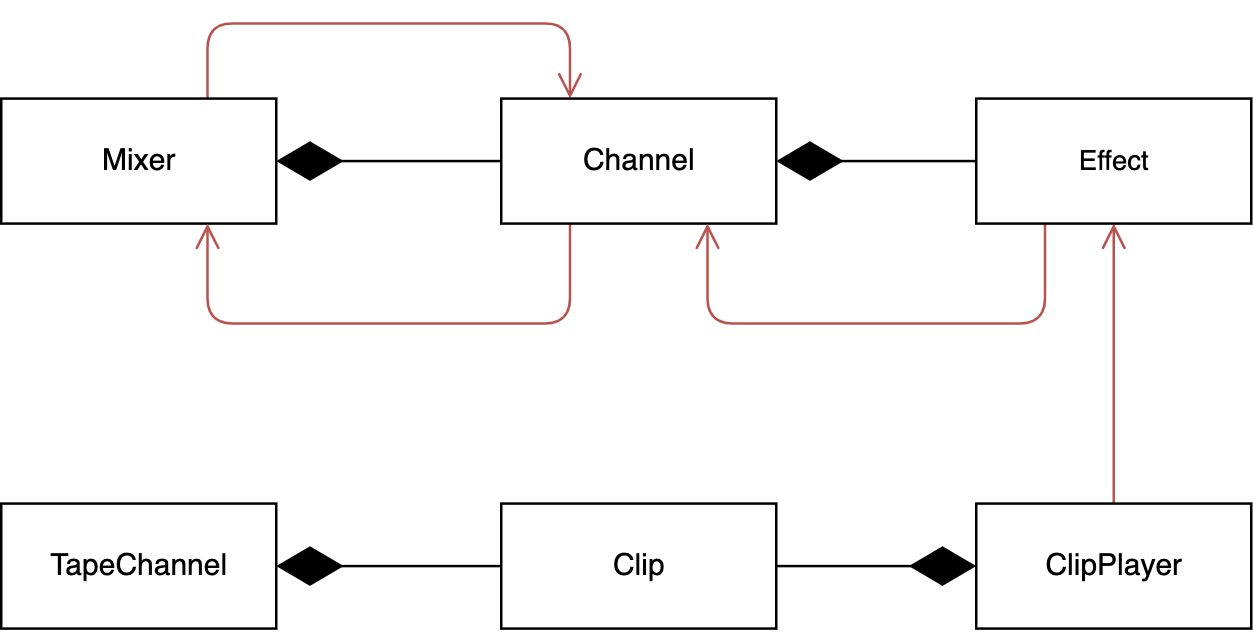
\includegraphics[scale=1.7]{img/domain.png}
\caption{Schema UML dell'analisi del problema, con rappresentate le entità principali ed i rapporti fra loro.}
\end{figure}

\subsection{Glossario termini}
\begin{center}
\begin{longtable}{| m{5em} | m{3.2cm}| m{7cm} |} 
 \hline
 \textbf{Termine} & \textbf{Analog/Digital} & \textbf{Descrizione} \\ [0.5ex] 
 \hline
 mono & A/D & Segnale audio unico che viene inviato sia al diffusore destro che al sinistro. \\ 
 \hline
 stereo & A/D & Segnale audio che contiene informazioni separate per il diffusore destro rispetto al sinistro.
Abbiamo quindi due segnali distinti. \\
 \hline
 mixer & A/D & Oggetto che riceve vari input audio e gestisce il percorso dei vari segnali  per poi sommarli assieme in uno o più uscite.
Un mixer può anche fornire all’utente equalizzatori, compressori o altri processori di segnale. \\
 \hline
 channel, canale & A/D & Un canale è una porzione del mixer che prende un input audio (mono o stereo), eventualmente lo processa, e poi fornisce l’audio ottenuto al mixer per sommarlo ad altri canali o indirizzare il segnale da qualche parte. \\
 \hline
 traccia & A/D & È comune pratica parlare di “traccia” per identificare un canale di un mixer. Con il termine traccia in realtà possiamo riferirci anche ad un file audio, per esempio nel caso del djing traccia = canzone. Nel caso di un mixer, la corretta dicitura è “canale”. \\ 
 \hline
 master & A/D & Canale del mixer che prende in input la somma dell’audio di tutti gli altri canali. L’out del master corrisponde all’uscita principale dell’audio del mixer. \\
 \hline 
 canale di ritorno, send/return, ausiliario, aux & A/D & Canale del mixer ausiliario che prende in input la duplicazione dell’uscita di altri canale principali allo scopo di processare il segnale in parallelo. \\
 \hline
 routing & A/D & Descrizione delle modalità di indirizzamento del segnale audio all’interno di un mixer. Più precisamente il percorso che il segnale percorre nel mixer. \\
 \hline
 clip & D & Porzione di contenuto di un canale modificabile singolarmente e posizionabile nella timeline. \\
 \hline
 timeline & D & Linea del tempo su cui posizionare le varie clip/contenuti. \\
 \hline
 MIDI & A/D & Musical Instrument Digital Interface.
Protocollo standard per l’interazione degli strumenti elettronici anche tramite computer. \\
\hline
clock & A/D & Un clock è un segnale che consente di sincronizzare il bitrate (il trasferimento dei singoli bit) di diverse macchine.
N.B.
Nel software l’oggetto Clock non scandisce il bitrate, ma il tempo per sincronizzare la riproduzione delle varie clip. \\
\hline
\end{longtable}
\end{center}

\chapter{Design}
Nella fase di design è stato necessario individuare i vari compiti e responsabilità da assegnare alle varie entità del modello.

Innanzitutto occorre distinguere le entità che lavorano con audio registrato da quelle che processano audio in tempo reale.
Le prime rappresentano i contenuti audio con tutte le informazioni necessarie al posizionamento nella timeline. Le seconde invece lavorano in tempo reale accettando uno stream audio in ingresso e processando i dati in tempo reale.
Se si vuole fare un parallelismo con il dominio analogico, il nastro memorizza in modo statico l’informazione audio, mentre i processori di segnale o il mixer ricevono un flusso audio e lo modificano in tempo reale fornendo poi in output il risultato.

Una seconda distinzione è quella tra entità che lavorano informazioni di alto livello rispetto a quelle che lavorano con informazioni di basso livello.
Infatti, per consentire all’applicazione di prendere decisioni e suggerire all’utente i corretti parametri o la corretta organizzazione del progetto, è necessario memorizzare informazioni aggiuntive a quelle strettamente necessarie per la gestione dell’audio.
Si distinguono le entità di basso livello che fanno parte dell’editing da quelle di alto livello che fanno parte del planning. Le seconde saranno utili al software per analizzare il progetto e fare scelte in modo consapevole.
Vi sono anche entità che hanno il compito di coordinare tra loro le entità di alto livello e quelle di basso livello, per esempio il Manager.
Quest’ultima è un'entità “intelligente”, che ha il compito di interpretare le informazioni disponibili ad alto e basso livello al fine di comandare le varie parti del modello e portare a termine le azioni richieste dall’utente in modi diversi in base allo stato corrente del progetto.

\parskip 0.8in
Vengono quindi introdotti alcuni concetti chiave per il modello:
\parskip 0in

\begin{center}
\begin{longtable}{| m{7em} | m{7cm} |} 
 \hline
 \textbf{Concetto} & \textbf{Descrizione} \\ [0.5ex] 
 \hline
 Clip & È un contenitore per un qualsiasi contenuto che si voglia aggiungere al progetto. Memorizza la propria durata e il contenuto da riprodurre in corrispondenza della clip. \\ 
 \hline
 Tape channel & Rappresenta la timeline per un canale audio. Memorizza le clip e la loro posizione nella timeline e controlla che non vi siano più clip sovrapposte nel tempo. \\
 \hline
 Clip player & Riproduce una clip fornendo in output un audio in tempo reale. \\
 \hline
 Recorder & Registra un flusso audio in ingresso in tempo reale (per esempio da un microfono). \\
 \hline
 Channel & Rappresenta un canale di un mixer.
Prende un flusso audio in ingresso, lo processa e restituisce in output il risultato. \\ 
 \hline
 Mixer & Contiene vari canali e gestisce il routing dell’audio. \\
 \hline 
 Effect & Processore di segnale. Prende un input audio, lo processa e restituisce un out con l’audio processato. \\
 \hline
 Processing unit & Catena di effetti per un canale. Prende un input audio, lo processa tramite diversi effetti e restituisce un out con l’audio processato. \\
 \hline
 Clock & Scandisce il tempo di playback per coordinare le varie parti dell’engine. \\
 \hline
 Part & Informazioni ad alto livello di una clip. \\
 \hline
 Role & Informazioni ad alto livello di un canale. \\
\hline
Section & Sezione della timeline decisa dall’utente per indicizzare una porzione del contenuto audio. \\
\hline
Timeline & Timeline di progetto che gestisce le informazioni ad alto livello. \\
\hline
Manager & Unisce le informazioni di alto e basso livello per prendere decisioni su come eseguire le azioni richieste dall’utente. \\
\hline
\end{longtable}
\end{center}

Segue un elenco con la classificazione delle entità appena descritte:
\begin{center}
\begin{longtable}{| m{10em} | m{5cm} | m{4cm} |} 
 \hline
 \textbf{Concetto} & \textbf{Real time/Non real time} & \textbf{Editing/Planning} \\ [0.5ex] 
 \hline
 Clip & Non real time & Editing \\ 
 \hline
 Tape channel & Non real time & Editing \\
 \hline
 Clip player & Real time & Editing \\
 \hline
 Recorder & Real time & Editing \\
 \hline
 Channel & Real time & Editing \\ 
 \hline
 Mixer & Real time & Editing \\
 \hline 
 Effect & Real time & Editing \\
 \hline
 Processing unit & Real time & Editing \\
 \hline
 Engine & Real time & Editing \\
 \hline
 Part & Non real time & Planning \\
 \hline
 Role & Non real time & Planning \\
\hline
 Section & Non real time & Planning \\
\hline
 Timeline & Non real time & Planning \\
\hline
 Manager & Non real time & Editing, Planning \\
\hline
\end{longtable}
\end{center}

\section{Architettura}
Per il software si è scelto un pattern architetturale di tipo MVC, opportunamente modificato per assecondare l’utilizzo di JavaFX che prevede l’utilizzo di classi controller “intermedie”. La classe del Manager nel model, che rappresenta l’applicazione in sé, viene interpellata dal Controller, che comunica con i controller di JavaFX. Ogni file FXML è associato ad un controller con i rispettivi listener. Questi controller chiamano il Controller principale che effettua le azioni sul manager e poi aggiorna la View. Dato che la view dell’applicazione è divisa in due parti, una di Planning e una di Edit, ed entrambe devono lavorare sullo stesso set di dati, è stata creata una classe ViewData che contiene tutti i dati che vanno rappresentati nella view stessa. Quindi il controller invece di aggiornare direttamente la view aggiorna i dati dentro ViewData e la view, tramite listener, si aggiorna in base ai dati presenti dentro di essa.

\begin{figure}[h]
\centering{}
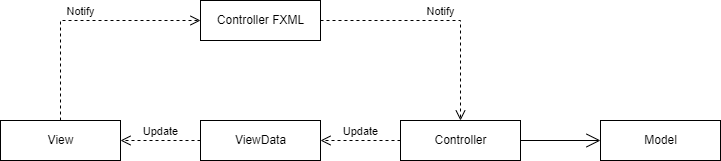
\includegraphics[width=\textwidth]{img/arch.png}
\caption{Schema UML architetturale di Resplan.}
\end{figure}

\section{Design dettagliato}

\subsection{Interazioni principali}
\subsubsection{Manager}
Ogni qualvolta l’utente richieda un’azione sul modello, la richiesta viene accolta dal manager. Questo analizza lo stato corrente dell’applicazione per identificare la modalità migliore per portare a termine il compito. A questo punto il manager può istanziare o modificare elementi di alto e basso livello.
Per mantenere i riferimenti tra gli oggetti di alto e basso livello vengono introdotti il ChannelLinker ed il ClipLinker. 
Per ogni canale vengono mantenuti dal ChannelLinker i riferimenti al Channel, al TapeChannel e al Role.
Il primo gestisce il flusso audio e il processing in tempo reale dell’audio che passa nel canale. Il secondo agisce come un nastro salvando le posizioni delle varie clip del canale nella timeline. Il terzo invece mantiene le informazioni di alto livello del canale, utili al manager per prendere decisioni.
Per ogni clip il ClipLinker mantiene unita la Clip di basso livello con la Part di alto livello.

\subsubsection{Non Real Time}
Viene istanziato un TapeChannel per ogni canale del mixer. Il tape channel gestisce le Clip al suo interno assicurandosi che le varie clip non si sovrappongano nel tempo. Qualsiasi modifica relativa alla posizione o alla durata della clip nella timeline viene effettuata per mezzo del TapeChannel.

\subsubsection{Real time}
Quando si vuole ascoltare in real time o renderizzare l’audio del progetto occorre azionare l’Engine. 
L’Engine per ogni clip del canale istanzia un ClipPlayer il cui output viene collegato all’input del corrispettivo Channel. Il canale indirizza l’audio all’interno della sua ProcessingUnit dove vari Effects processano l’audio. Infine il Mixer si occupa del routing tra i vari canali sommando l’audio in uscita in un unico canale master. L’output del canale master viene poi inviato all’uscita audio di sistema per la riproduzione.
Una volta azionato, l’Engine si occuperà di azionare i clip player nel momento opportuno facendo di fatto partire la riproduzione delle clip nell’istante corrispondente alla loro posizione nella timeline.

\subsection{Alessandro Antonini}

\subsubsection{RPClip, RPClipPlayer e RPTapeChannel}
Una delle prime entità da modellare è stata la clip, fondamentale per aggiungere contenuti al progetto.
Inizialmente per le clip sono stati individuati i seguenti requisiti: 
\begin{itemize}
    \item memorizzare il proprio contenuto;
    \item salvare la sua durata e posizione nella timeline;
    \item possibilità di specificare la sezione del contenuto da riprodurre, nel caso il contenuto sia più lungo della durata della clip;
    \item evitare la sovrapposizione nel tempo di più clip nello stesso canale;
    \item riprodurre il proprio contenuto.
\end{itemize}

Dopo un’attenta analisi è emerso che alcune di queste responsabilità potevano essere trasferite ad oggetti diversi. 
Si nota infatti che i metodi relativi alla riproduzione verranno chiamati dall’Engine, mentre quelli per il posizionamento nella timeline verranno chiamati dal Manager.
I metodi inerenti alla Clip sono invece quelli riguardanti la propria durata e il contenuto.
Sono state create interfacce diverse per i vari “client” e sono state separate le responsabilità per non violare il single responsibility principle.
Con la nuova suddivisione dei compiti l’interfaccia RPTapeChannel permette di posizionare degli oggetti RPClip ed effettuare controlli riguardanti la sovrapposizione nella timeline.
L’interfaccia RPClipPlayer conterrà invece i metodi per riprodurre il contenuto della clip.
Oggetti di tipo RPTapeChannel verranno utilizzati dal Manager, mentre gli RPClipPlayer saranno utilizzati dall’Engine.

\begin{figure}[H]
\centering{}
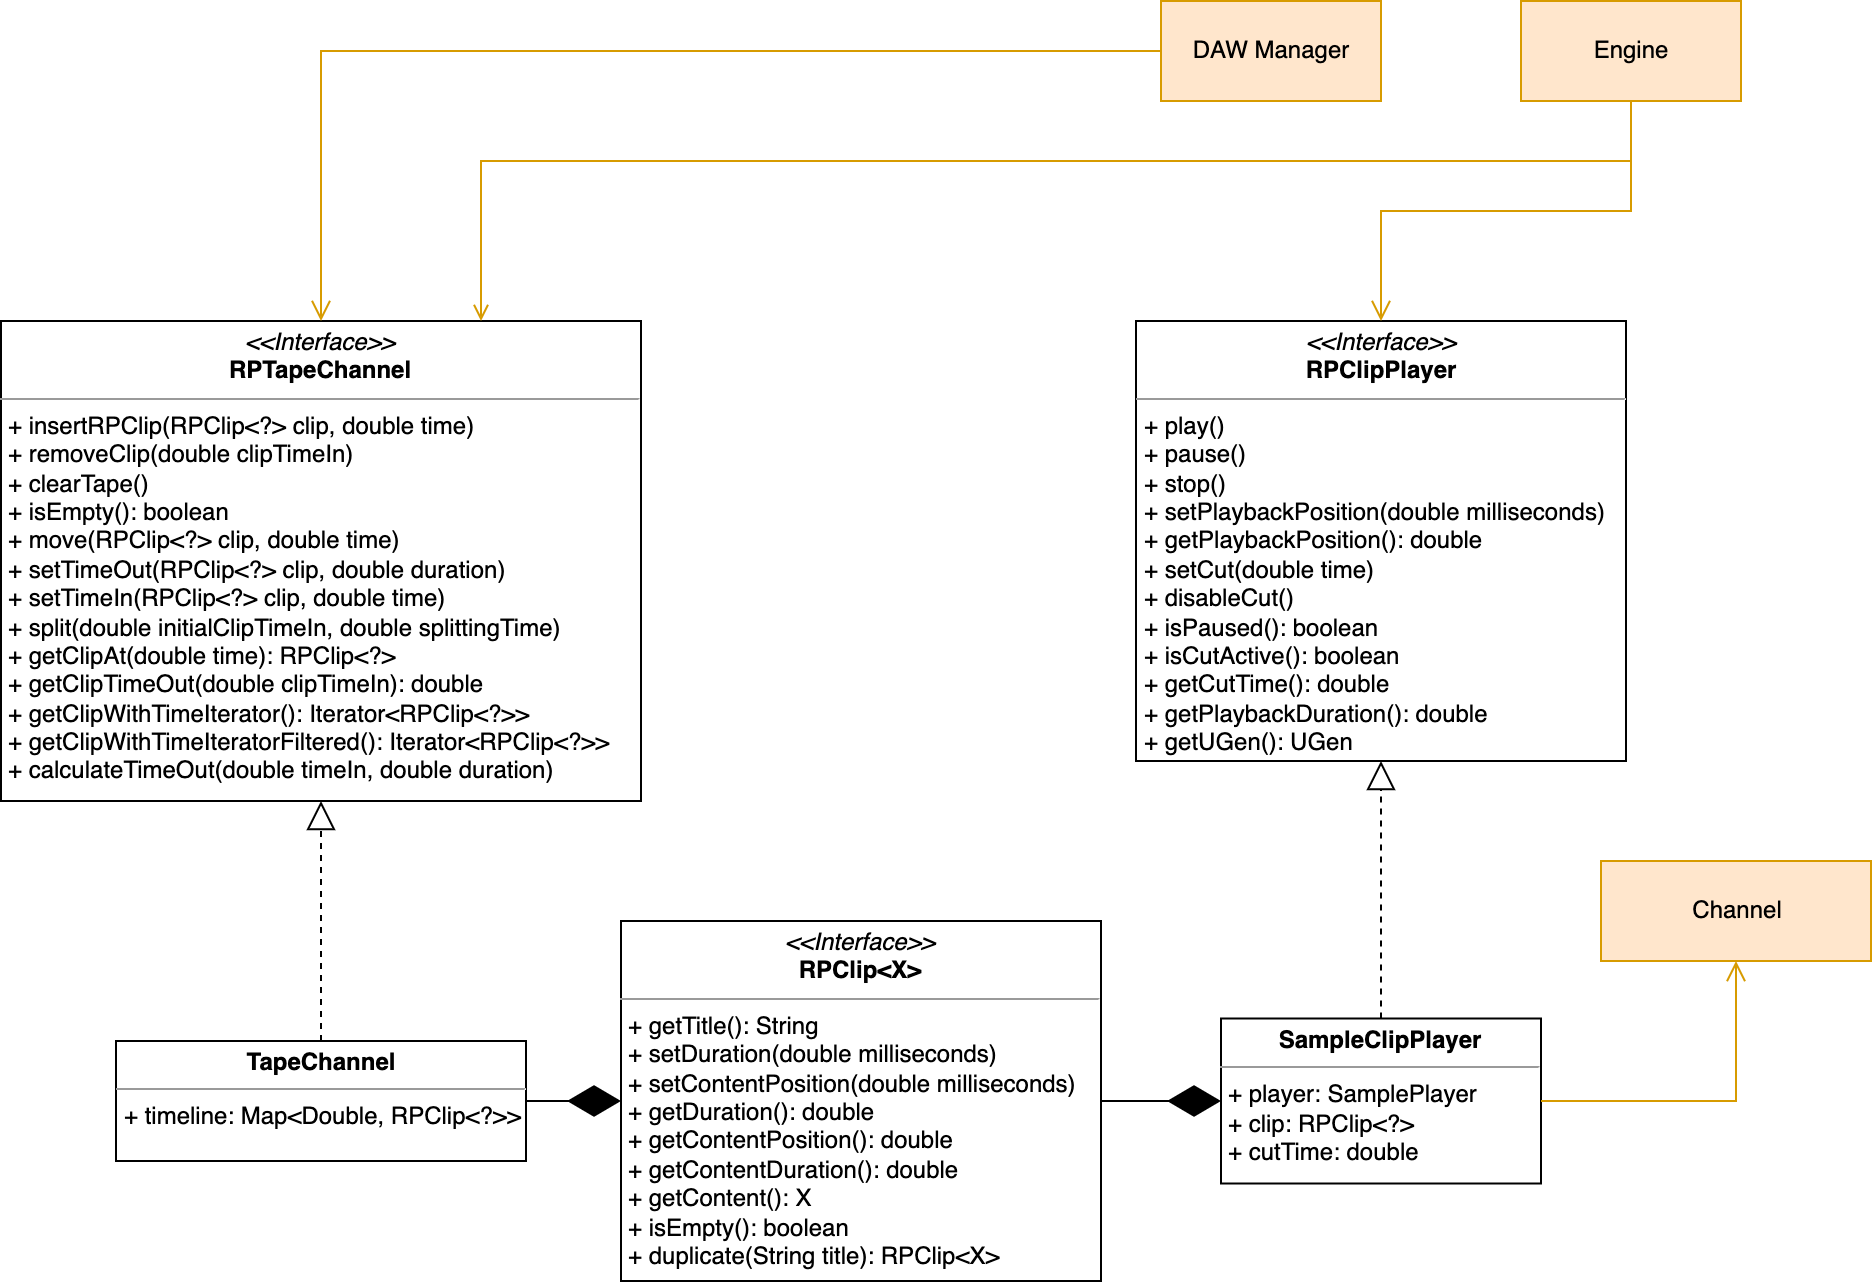
\includegraphics[width=\textwidth]{img/tapechannel.png}
\caption{UML che mostra l'interazione tra TapeChannel, Clip ed elementi esterni.}
\end{figure}

\subsubsection{Clip proxy}
Per le Clip un requisito necessario è quello di lavorare con tipi diversi di contenuto. In particolare Resplan prevede la possibilità di lavorare con clip di file audio oppure con clip vuote, quindi senza contenuto. Si vuole lasciare però la possibilità di aggiungere in futuro nuovi tipi di contenuto, per esempio clip di file MIDI.

Una prima idea è stata quella di utilizzare i generici nell’interfaccia RPClip. Tuttavia questa soluzione risolve solo in parte il problema in quanto per diversi contenuti sarebbero stati necessari controlli diversi, mentre parte del codice sarebbe stato duplicato per clip di tipologie differenti.
La necessità di effettuare controlli in base al tipo di contenuto ha fatto preferire l’utilizzo del pattern proxy.
L’EmptyClip diventa l’implementazione base dell’RPClip, mentre SampleClip “wrappa” l’EmptyClip per effettuare i controlli sulla durata del contenuto audio (il file audio non può essere più breve della clip).
Tuttavia sarebbe stato anche necessario controllare che il file assegnato alla clip fosse un file esistente, pertanto, anche ai fini di facilitare l’implementazione futura di nuove tipologie, è stato introdotto un nuovo stadio di proxy con l’aggiunta della classe FileClip che rappresenta una clip con un qualsiasi file come contenuto.
In seguito l’interfaccia RPClip è stata comunque resa generica per poter lavorare con il contenuto della clip della classe giusta.

\begin{figure}[H]
\centering{}
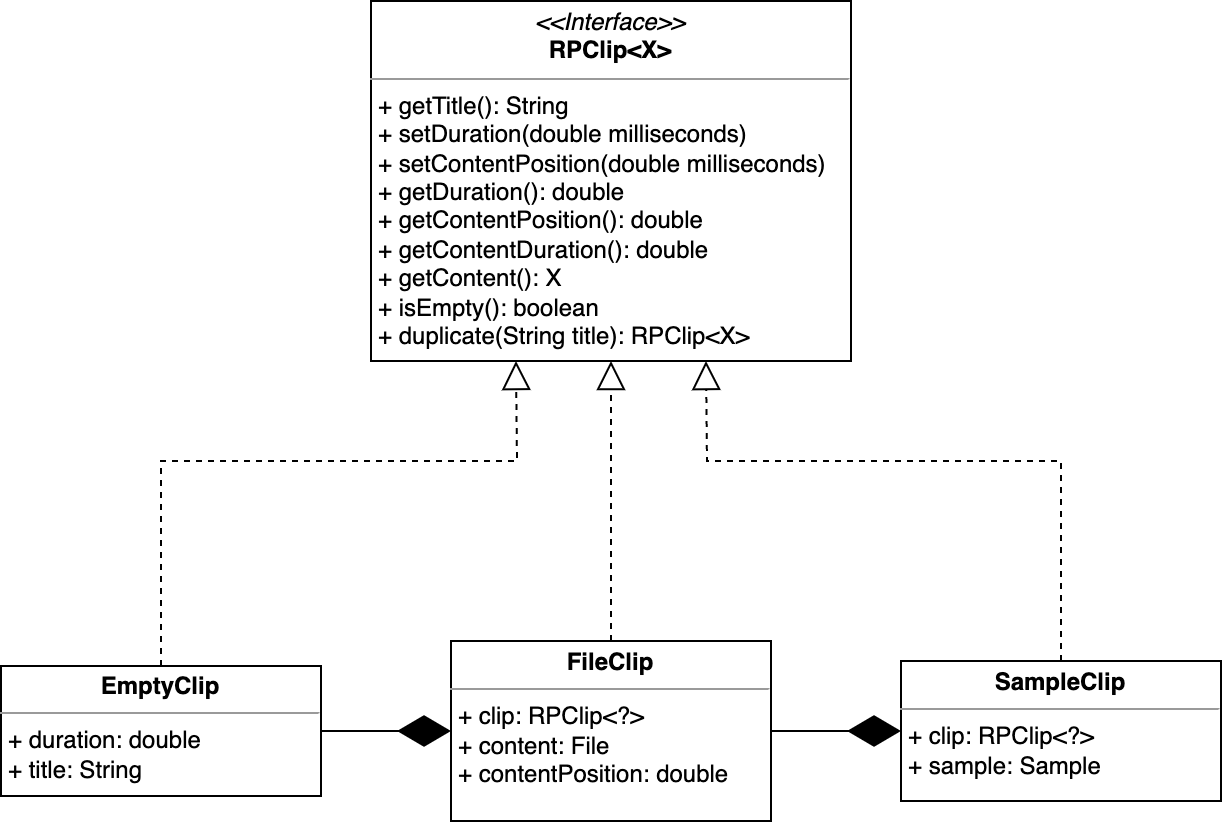
\includegraphics[width=\textwidth]{img/clip.png}
\caption{Gerarchia di Clip con sue implementazioni.}
\end{figure}

\subsubsection{RPTapeChannel}
Il compito di tenere la posizione delle clip nella timeline per un determinato canale è stato affidato alla classe TapeChannel, implementazione dell’interfaccia RPTapeChannel. Un oggetto TapeChannel si assicura che le clip siano posizionate in maniera corretta, senza sovrapposizioni temporali.
L’interfaccia implementata fornisce i metodi per spostare e ridimensionare le clip e definire la posizione del contenuto, oltre che aggiungere o rimuovere clip dal TapeChannel.
Inoltre sono stati aggiunti due metodi per ottenere un iteratore delle clip del TapeChannel con il rispettivo tempo. Entrambi restituiscono un Iterator\begin{math}<\end{math}Pair\begin{math}<\end{math}Double, RPClip\begin{math}<\end{math}?\begin{math}>>>\end{math}, ma il secondo, come previsto dal pattern strategy, accetta in input un'interfaccia funzionale Predicate per filtrare le clip che l’Iterator dovrà restituire.

\subsubsection{RPClipPlayer}
Esistendo implementazioni diverse delle RPClip in base al contenuto, servono anche ClipPlayers diversi in base al tipo di contenuto della clip.
I ClipPlayers sono stati concepiti come oggetti usa e getta che vengono creati al momento del bisogno dall’Engine. È stata quindi implementata una factory di SampleClipPlayers, che al momento sono l’unica tipologia di clip che è possibile riprodurre. In futuro sarà possibile implementare delle factory per ogni nuovo tipo di player e aggiornare l’Engine per istanziare players del tipo giusto in base alla clip da riprodurre.

Per quanto riguarda i players è stato necessario introdurre il “cut time”:
il punto della clip da cui un player deve far partire la riproduzione.
Il cut time non corrisponde alla content position, infatti quest’ultima definisce il punto da cui deve iniziare la riproduzione del contenuto della clip in corrispondenza del suo inizio. Il cut time invece viene utilizzato dall’Engine che quando crea i player vuole momentaneamente spostare il punto in cui far partire la riproduzione della clip, per esempio quando l’utente vuole far partire la riproduzione da un tempo della timeline che taglia a metà una clip.

\begin{figure}[H]
\centering{}
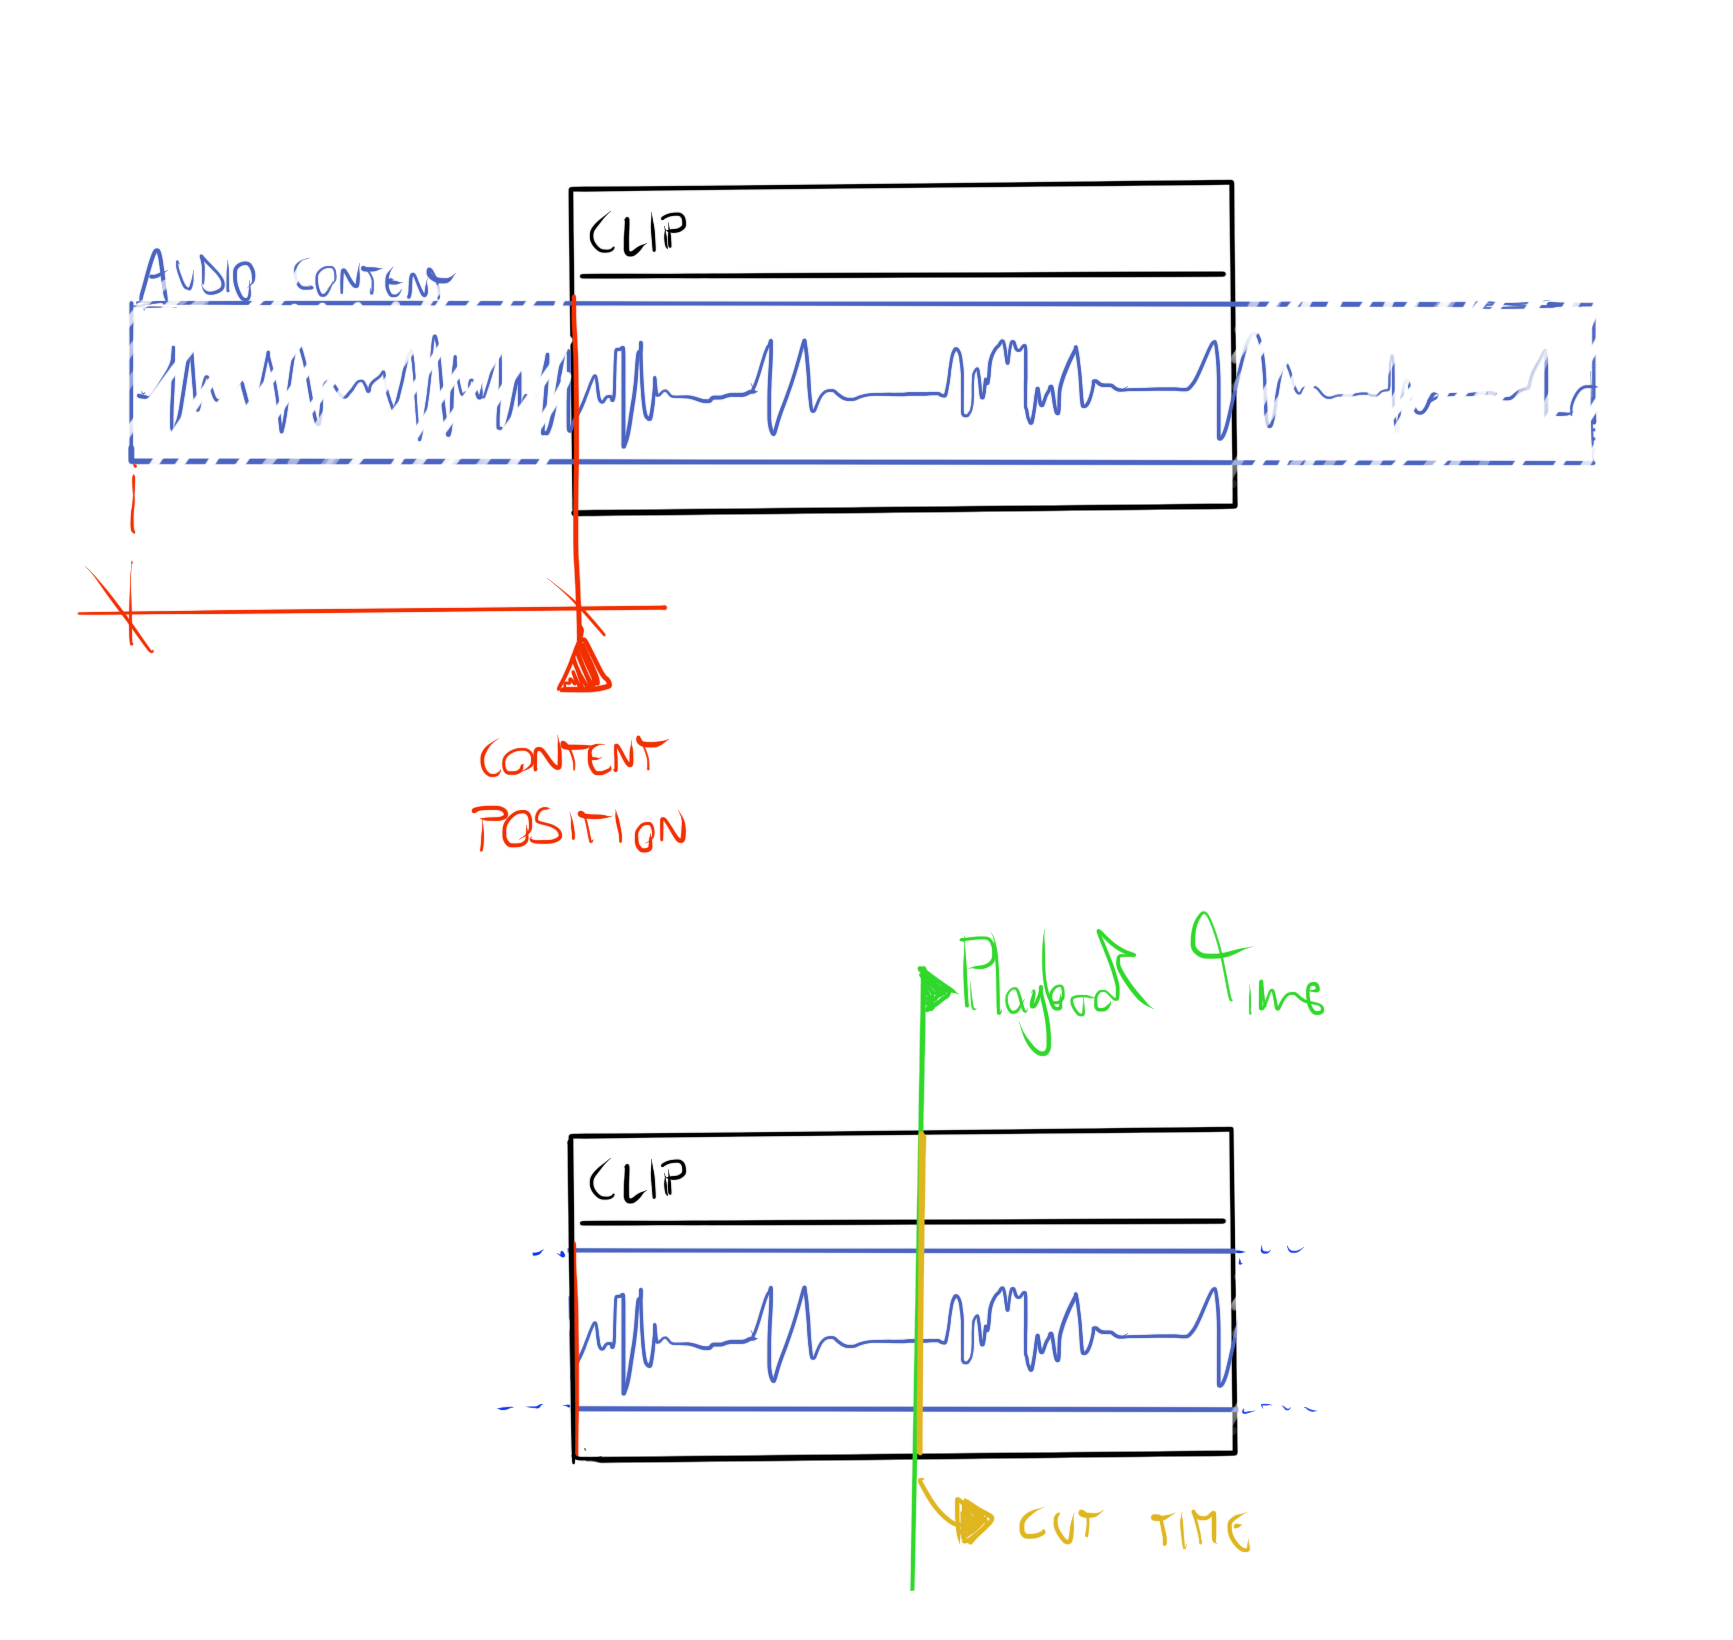
\includegraphics[scale=0.27]{img/clipModel.png}
\caption{Rappresentazione di content position e cut time}
\end{figure}

Nell'interfaccia SamplePlayerFactory sono disponibili due metodi: uno per creare un player con il cut time disattivato, l’altro per crearne uno con un cut time attivo.

\begin{figure}[H]
\centering{}
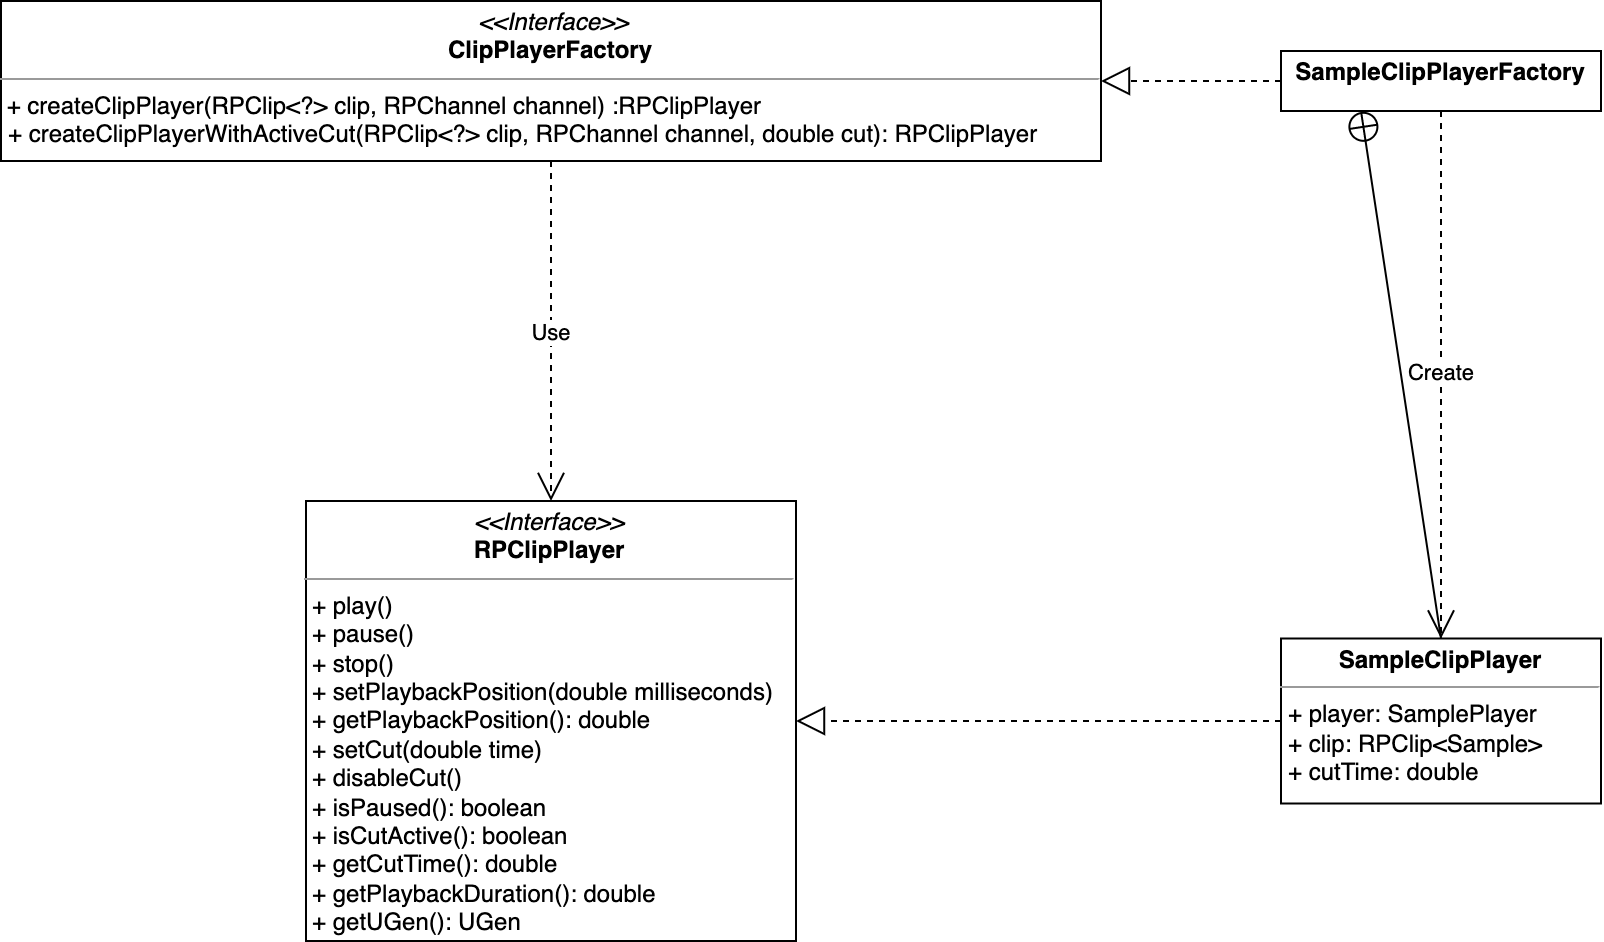
\includegraphics[width=\textwidth]{img/clipplayer.png}
\caption{UML che mostra il funzionamento di ClipPlayerFactory.}
\end{figure}

\subsubsection{RPEngine}
L’Engine deve occuparsi della riproduzione delle clip esistenti nella timeline.
L’interfaccia RPEngine pertanto avrà i seguenti metodi:
\begin{itemize}
    \item start()
    \item pause()
    \item stop()
    \item setPlaybackTime(Double time)
    \item getPlaybackTime()
    \item isPaused()
\end{itemize}
Anche nell’Engine, così come per le Clip, sono state trovate responsabilità diverse, che sono state pertanto divise tra varie sottoclassi.
Si rende necessario un Clock generale che scandisce il tempo per sincronizzare la riproduzione delle varie clip.
Il Clock va avanti a step interi ed ogni step equivale a un intervallo di tempo trascorso (CLOCK\_STEP\_UNIT).
Il Clock avrà un metodo per incrementare uno step alla volta e per settare il tempo ad un time specifico oltre a quelli per ottenere il tempo corrente.
È stata poi creata Clock.Utility, una classe di utility innestata statica, che dovrà occuparsi della conversione da time a step e viceversa.
Inoltre serve un ClipPlayerNotifier che tramite il pattern observer notifica i vari player nel momento in cui devono partire o fermarsi.
La creazione e registrazione dei vari player al ClipPlayerNotifier avviene grazie al PlayersMapBuilder, il quale tramite la SamplePlayerFactory e il ChannelLinker crea una mappa in cui per ogni “time in” di una SampleClip viene creato e associato il SamplePlayer corrispondente.
Come spiegato nella sezione relativa ai ClipPlayer, qualora vengano introdotti nuovi tipi di clip sarà possibile filtrare le diverse tipologie ed utilizzare la giusta factory per istanziare l’implementazione corretta dei player.
Ovviamente serve una componente attiva che si occupi di aggiornare il clock ad ogni CLOCK\_STEP\_UNIT. Il compito viene affidato ad una nuova classe che estende Thread: Conductor.

\subsubsection{Risoluzione delle problematiche relative all’implementazione dell’Engine}
L’Engine è stato uno degli elementi del modello più complessi da implementare. Infatti sviluppare un Engine efficiente si traduce nel dover gestire concetti relativi al tempo, all’interazione tra thread, e alla sincronizzazione di vari oggetti.

La prima considerazione da fare è che il clock deve avanzare a step. Infatti non è possibile gestire un aggiornamento continuo nel tempo, ma la classe Conductor può aggiornare il clock solo in maniera periodica, chiamando il metodo step() ad intervalli regolari di tempo.
\paragraph{N.B.}
In realtà anche nei TapeChannel non vi sono infiniti valori a cui le clip possono essere registrate, in quanto la precisione rimane al millesimo di secondo. Tuttavia non è comunque possibile aggiornare ogni millesimo di secondo il Clock in quanto il lavoro richiederebbe un utilizzo eccessivo di risorse da parte del thread.
\parskip 0.2in

La soluzione più naturale è stata quella di introdurre la CLOCK\_STEP\_UNIT, che è la quantità di tempo corrispondente ad ogni step. In questo modo al passare di ogni CLOCK\_STEP\_UNIT il thread Conductor deve aggiornare il clock.
Inoltre per ottenere una riproduzione il più fedele possibile il tempo corrispondente alla CLOCK\_STEP\_UNIT verrà calcolato in base al sample rate utilizzato dal dispositivo audio in uso.
\parskip 0in

Questa soluzione introduce però alcune problematiche. La prima riguarda il pattern observer responsabile di azionare i ClipPlayers. Infatti i ClipPlayers vengono associati nella PlayersMap a chiavi corrispondenti al tempo di inizio della relativa Clip nella timeline. Tuttavia il clock non copre tutte le possibili chiavi della mappa in quanto avanza a step superiori al millisecondo, e quindi salta alcuni tempi.
Il rischio è che alcuni ClipPlayers non vengano notificati e non inizino la riproduzione della propria Clip.
Le soluzioni per tale problematica possono essere multiple. Considerando che non è possibile cambiare il metodo di aggiornamento del clock in uno che copra tutti i tempi, le possibili soluzioni sono: 
\begin{itemize}
    \item cambiare il PlayersMapBuilder per far si che i ClipPlayers vengano registrati su step esistenti,
    \item modificare il ClipPlayerNotifier in modo che vengano notificati tutti i ClipPlayers che sono registrati a tempi tra lo step precedente e quello attuale.
\end{itemize}
Dato che la classe Clock.Utility fornisce già metodi per la conversione da tempo a step esistenti, è stato scelto il primo approccio. Le PlayersMap non mappano più i players a dei tempi, ma ai corrispettivi step.
Tale soluzione sembra migliore anche analizzando il modello con una visione di alto livello, infatti grazie a questa modifica tutto l’Engine viene sincronizzato sulla base degli step, mentre il concetto di tempo viene eliminato dal meccanismo per il playback. La conversione in tempo rimane solamente per consentire l'interazione con la timeline e la posizione delle clip.

La seconda problematica emersa riguarda la conversione da Double in Long, che sono i tipi di dati utilizzati per memorizzare rispettivamente i tempi e gli step.
Quando ci si avvicina a numeri molto grandi di step, si rischia di non poter convertire i Long in un valore compreso nel range del dato Double. Per il dominio del programma non è necessario lavorare con numeri vicini ai limiti del range del dato Long (che interpretati come millisecondi superano il secolo). Viene quindi introdotto un CLOCK\_MAX\_TIME. 
Per il CLOCK\_MAX\_TIME è stato deciso un valore vicino a quello della durata di un anno. In questo modo l’utente non percepirà alcuna limitazione visto che nessun contenuto audio si avvicina a tale durata, al tempo stesso si rimane lontani dai valori Double/Long problematici.

Se sulla carta le problematiche dovevano essere risolte, nel momento del testing sono stati individuati ulteriori “bug” dell’Engine.
Il problema in questo caso persiste nel tempo di aggiornamento del clock. 
Il tempo di sleep del Conductor, che coincide alla CLOCK\_STEP\_UNIT, non corrisponde alla frequenza di aggiornamento del clock in quanto ad ogni ciclo il tempo di esecuzione delle istruzioni nel corpo del thread si aggiunge a quello dello sleep. Il risultato è che il tempo del programma scorre più lento di quello reale.
Per risolvere tale problematica la soluzione più immediata è stata quella di fornire al Clock il tempo esatto ad ogni aggiornamento, che il Conductor può calcolare grazie alla classe di libreria java.lang.System.
Questa modifica introduce nuovamente la problematica del salto di alcuni step. Si rende quindi necessario modificare il ClipPlayerNotifier per notificare anche i ClipPlayers degli step mancati. Ora ad ogni aggiornamento del Clock il ClipPlayerNotifier avvia tutti i player tra lo step precedente e il nuovo step.
Tale decisione purtroppo vanifica in parte lo sforzo che è stato fatto per mantenere separati i concetti di tempo e di step nell’Engine. Tuttavia per una soluzione diversa sarebbe necessario del tempo supplementare per indagare meglio sulla causa del rallentamento della frequenza di aggiornamento e studiare una soluzione ad-hoc migliore.

\subsubsection{PlayersMap e ClipPlayerNotifier}
Finora è stata descritta la versione finale dell’Engine, tuttavia in una prima implementazione gli observers del ClipPlayerNotifier non venivano mantenuti da una PlayersMap, ma direttamente dall’Engine e di conseguenza l’aggiornamento degli observers avveniva chiamando un metodo di quest'ultimo. 
Solo in seguito è stata eseguita una rifattorizzazione al fine di togliere all’Engine la responsabilità di gestire gli observers e preservare quindi il single responsibility principle.

Nella versione ultimata vengono introdotte la MapToSet e la PlayersMap. 
La prima è un potenziamento della java.util.Map. Questa nuova interfaccia generica che lavora con tipi di dati \begin{math}<\end{math}X,Y\begin{math}>\end{math} permette di mappare per ogni key di tipo X un Set \begin{math}<\end{math}Y\begin{math}>\end{math} di elementi.
La PlayersMap invece non è altro che un “wrapping” di una MapToSet dove le chiavi rappresentano degli step e per ogni step sono mappati i players di cui avviare la riproduzione.
Ogni volta che viene richiesto di far partire il playback l’Engine crea un nuovo ClipPlayerNotifier a cui passa nel costruttore una PlayersMap aggiornata.
Il compito di creare la PlayersMap viene affidato al PlayersMapBuilder, il quale grazie al pattern creazionale builder è in grado di riempire la nuova PlayersMap passo passo creando e inserendo tutti i ClipPlayers necessari e della corretta tipologia.

\begin{figure}[H]
\centering{}
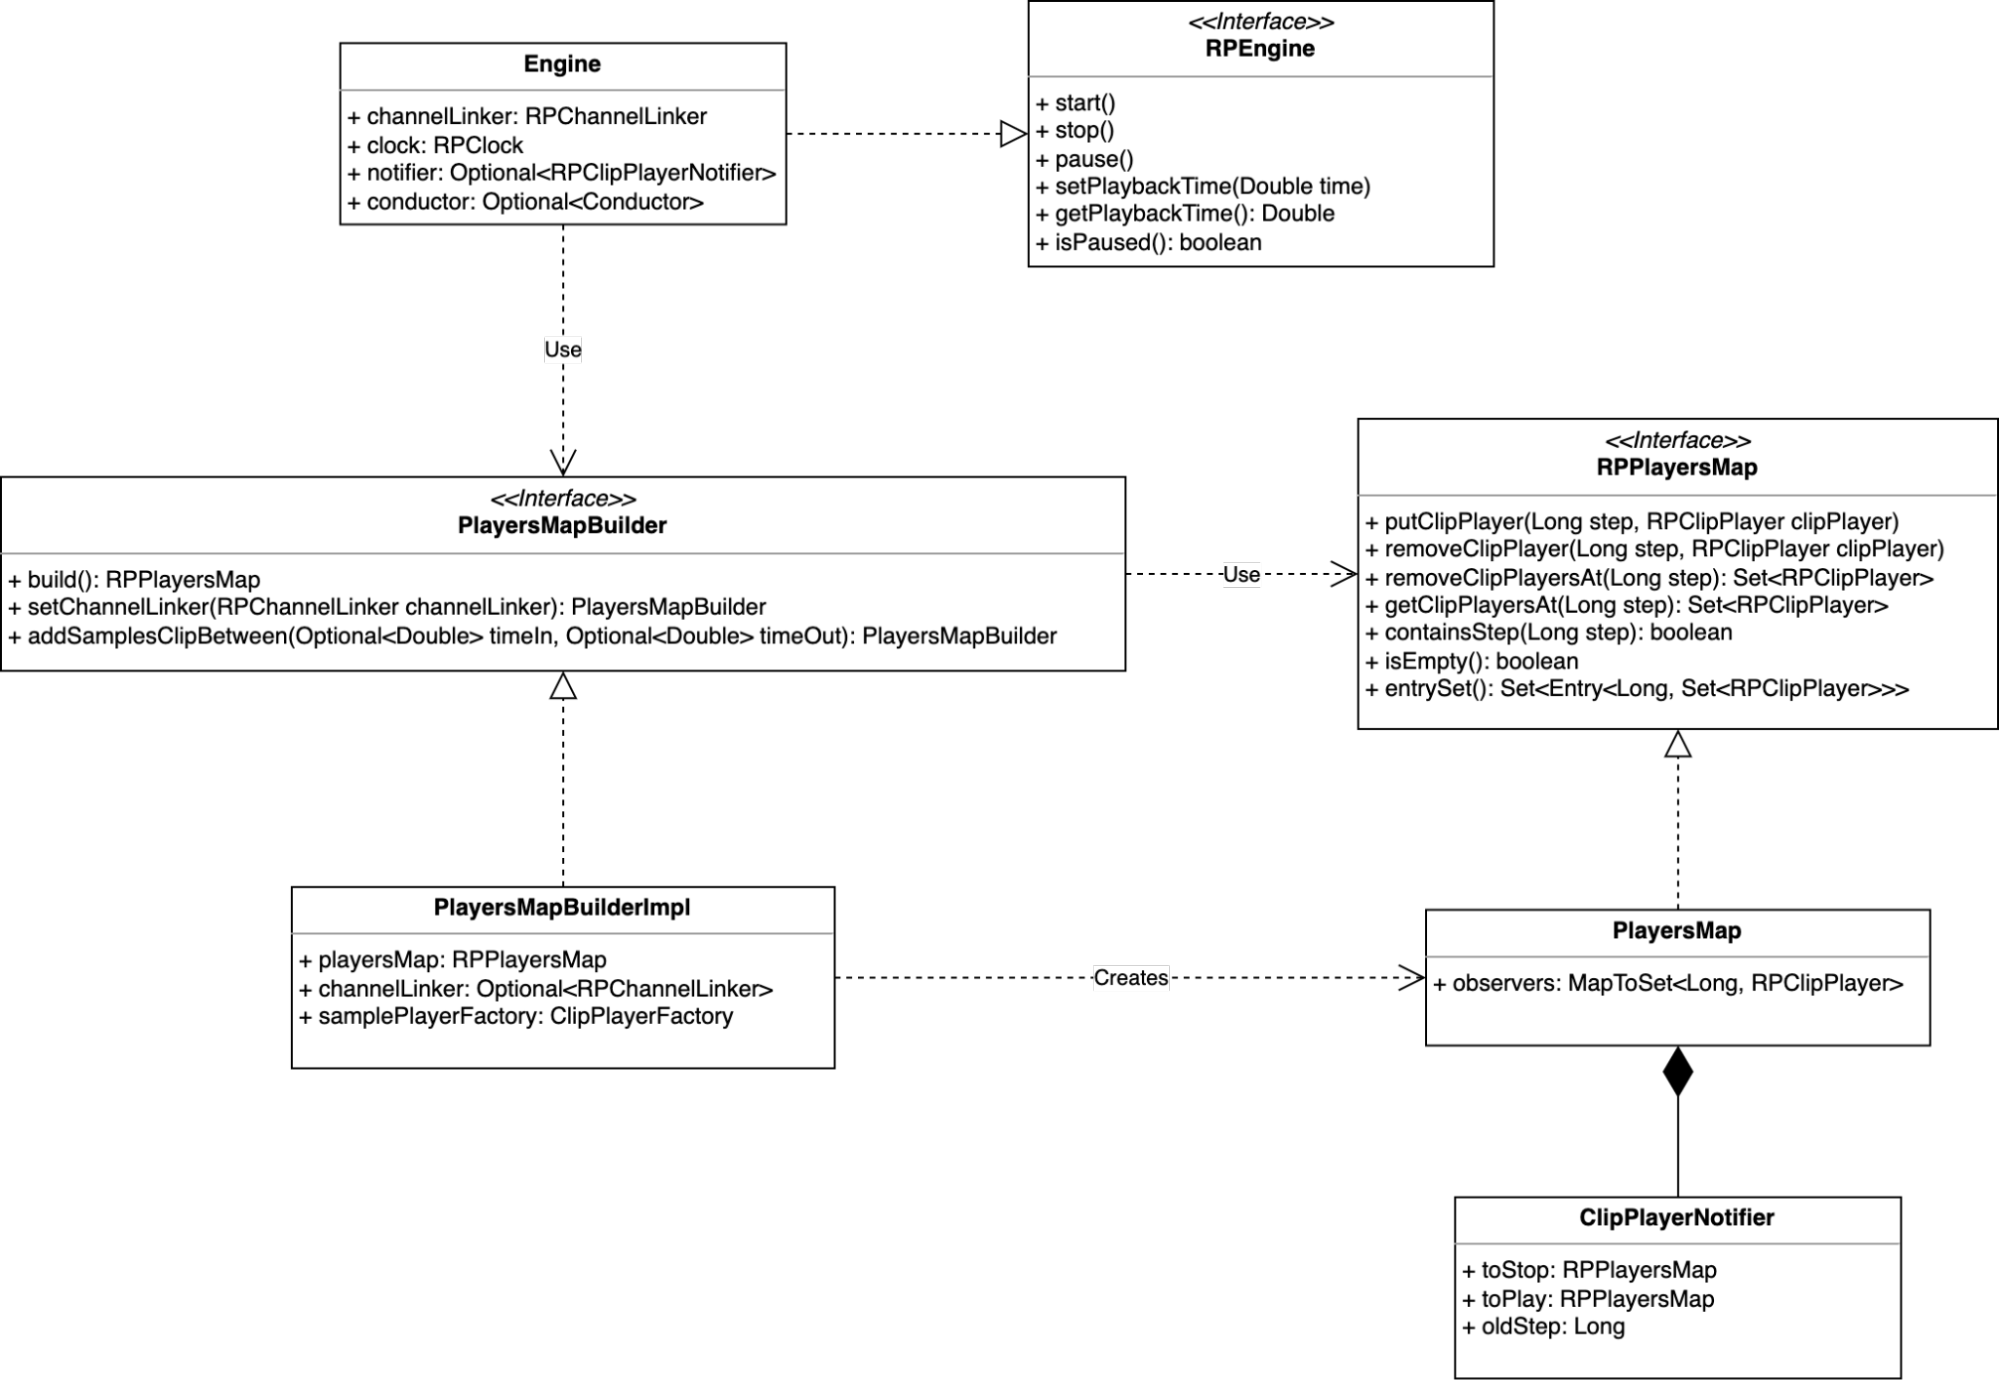
\includegraphics[width=\textwidth]{img/engine.png}
\caption{UML che rappresenta l'interazione di Engine con PlayersMapBuilder.}
\end{figure}

Rimane da gestire l’arresto dei vari ClipPlayers che vanno quindi notificati anche quando si vuole stoppare la riproduzione di una Clip.
Il ClipPlayerNotifier ogni volta che avvia un ClipPlayer iscrive lo stesso in una nuova PlayersMap. Tuttavia in quest’ultima i ClipPlayers verranno associati allo step in cui vanno arrestati.
Ora ad ogni aggiornamento del Clock il ClipPlayerNotifier notifica tutti gli observers iscritti per essere avviati o stoppati.

\begin{figure}[H]
\centering{}
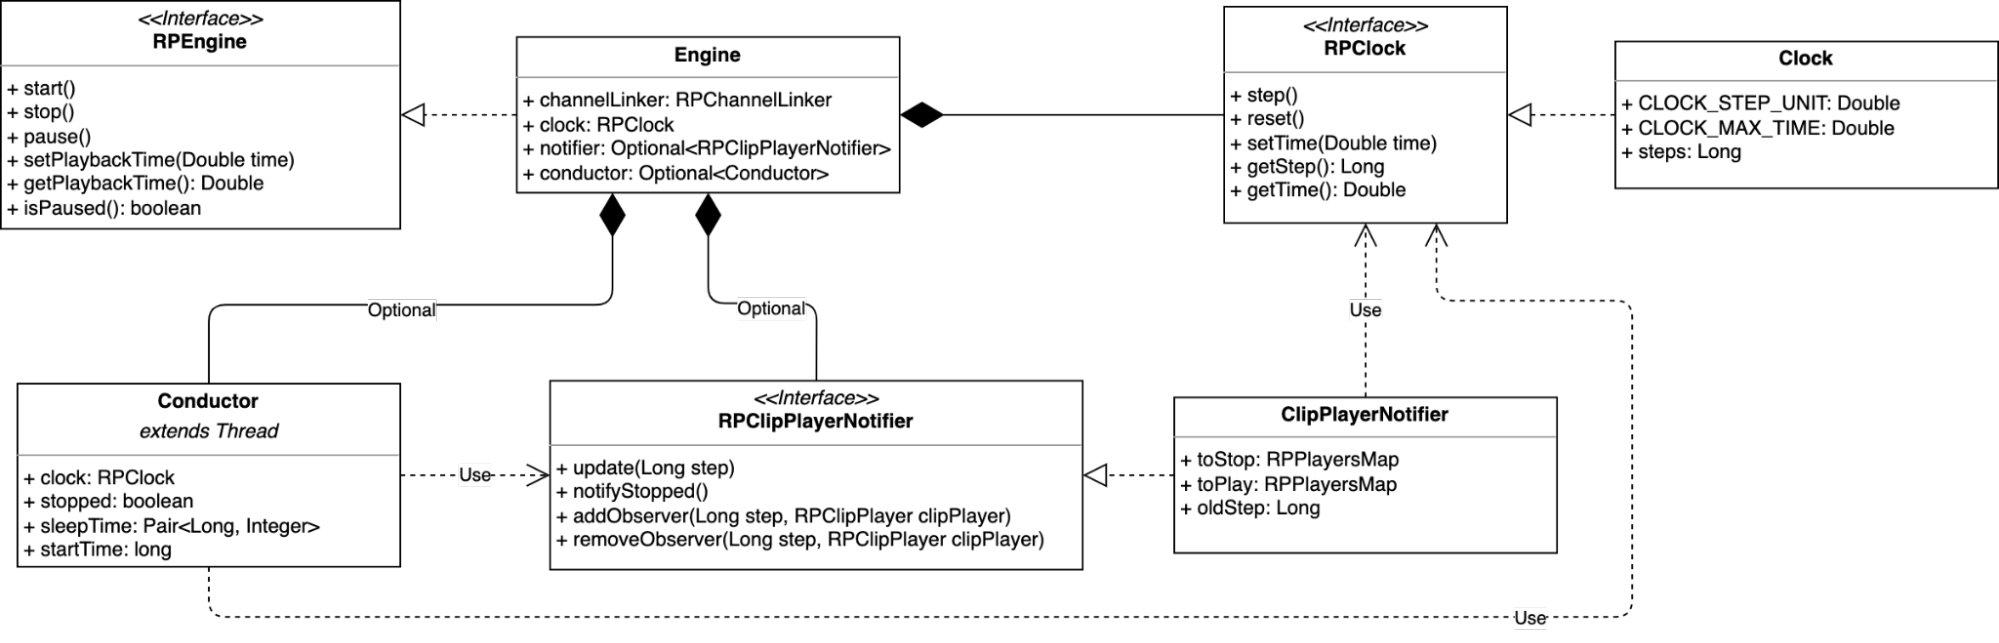
\includegraphics[width=\textwidth]{img/clock.png}
\caption{UML di Clock e ClipPlayerNotifier.}
\end{figure}

\subsection{Gabriele Menghi}
\subsubsection{Estrapolazione di concetti comuni}
Il mio compito all’interno del gruppo è stato quello di rappresentare all’interno del software gli elementi costituenti la DAW, ma ad alto livello, analizzandoli sotto l’aspetto organizzativo e non sotto quello dell’audio.

Per prima cosa ho notato subito la similarità tra gran parte degli elementi che avrei dovuto realizzare. Per quanto fossero concettualmente diversi, presentavano diversi aspetti in comune. Per risolvere nella maniera migliore questo problema ho deciso quindi di utilizzare il pattern “Strategy”, in modo da semplificare ed alleggerire il codice, ma soprattutto in modo da renderlo estensibile e riutilizzabile, dato che avendo un’interfaccia madre (“Element”), in caso di aggiunte, sarebbe stato necessario soltanto effettuare le opportune modifiche nell’interfaccia madre e successivamente implementare i nuovi metodi delle classi che implementano le interfacce che estendono da quella comune.

Non si è deciso invece di implementare prima i metodi  comuni e poi estendere una classe concreta comune, perché nonostante alleggerisse ancora di più il codice non sarebbe stata in grado di accettare piccole differenze nelle varie implementazioni in classi diverse, cosa che invece è possibile fare con la strategia adottata, rispettando comunque il contratto espresso dai metodi. 

\begin{figure}[h]
\centering{}
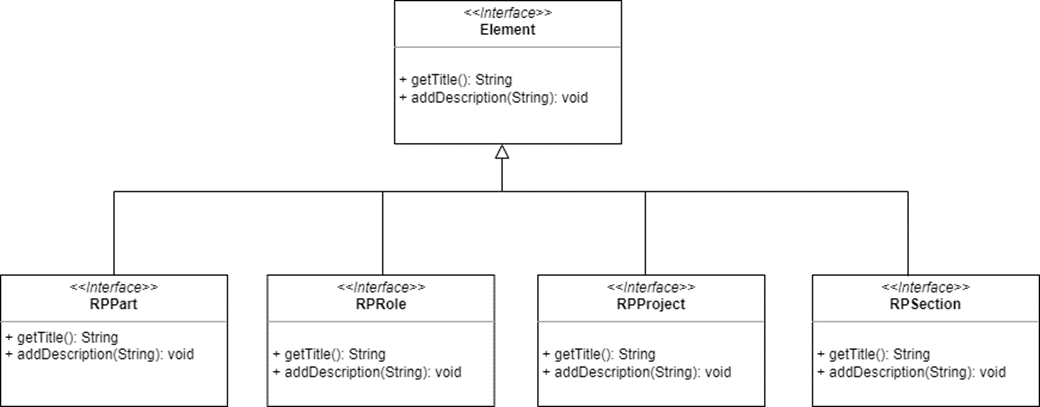
\includegraphics[width=\textwidth,scale=1]{img/element.png}
\caption{UML rappresentante il pattern Strategy sull’interfaccia “Element”.}
\end{figure}

\subsubsection{Parti e ruoli con aspetti in comune ed altri che li differenziano}
Addentrandoci più nello specifico, il problema successivo è costituito dalla rappresentazione di alcuni elementi che possiedono tipi. Gli elementi sono comuni tra loro, eccetto che a seconda della tipologia possiedono alcuni comportamenti distinti (e.g. una parte, che rappresenta una clip di alto livello, può contenere del testo solo se di tipo “speech”, ma come gli altri tipi di parti devono possedere un titolo ed una descrizione).

La mia decisione è stata quindi quella di rappresentare per prima cosa una generica parte attraverso un’interfaccia, ed in seguito di sfruttare il “Template Method” per realizzare una classe astratta che implementa i metodi comuni a tutte le tipologie di parti, e lascia invece l’implementazione dei metodi specifici alle classi concrete che estendono da lei.

Sfruttando questa soluzione, risultano più metodi template, ma si ottiene come risultato finale un codice più compatto, mano ripetitivo e più chiaro, e facilmente estensibile con nuove classi concrete che si basino su quella astratta comune.

\begin{figure}[h]
\centering{}
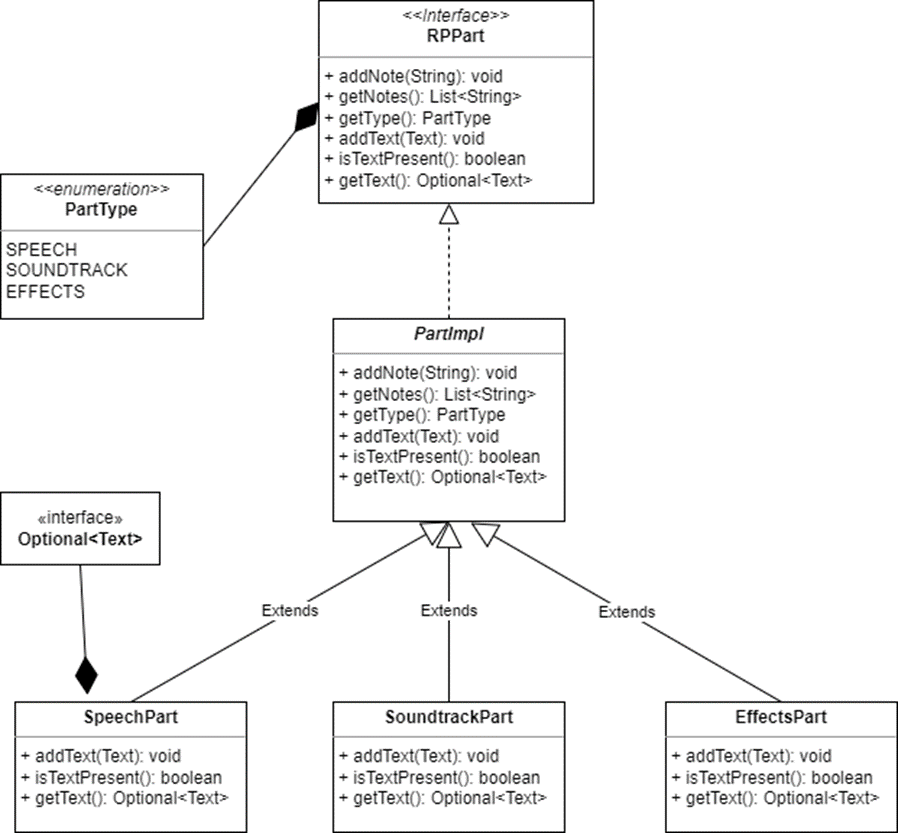
\includegraphics[width=\textwidth,scale=1]{img/part.png}
\caption{UML rappresentante Template Method sulla classe astratta “PartImpl”.}
\end{figure}

Discorso analogo si può effettuare per l’elemento RPRole, che di nuovo, a seconda della tipologia, presenta o meno certe caratteristiche. Questa volta, se il role, che rappresenta un canale di alto livello, è della tipologia “Speech”, gli può essere associato uno speaker.

\begin{figure}[h]
\centering{}
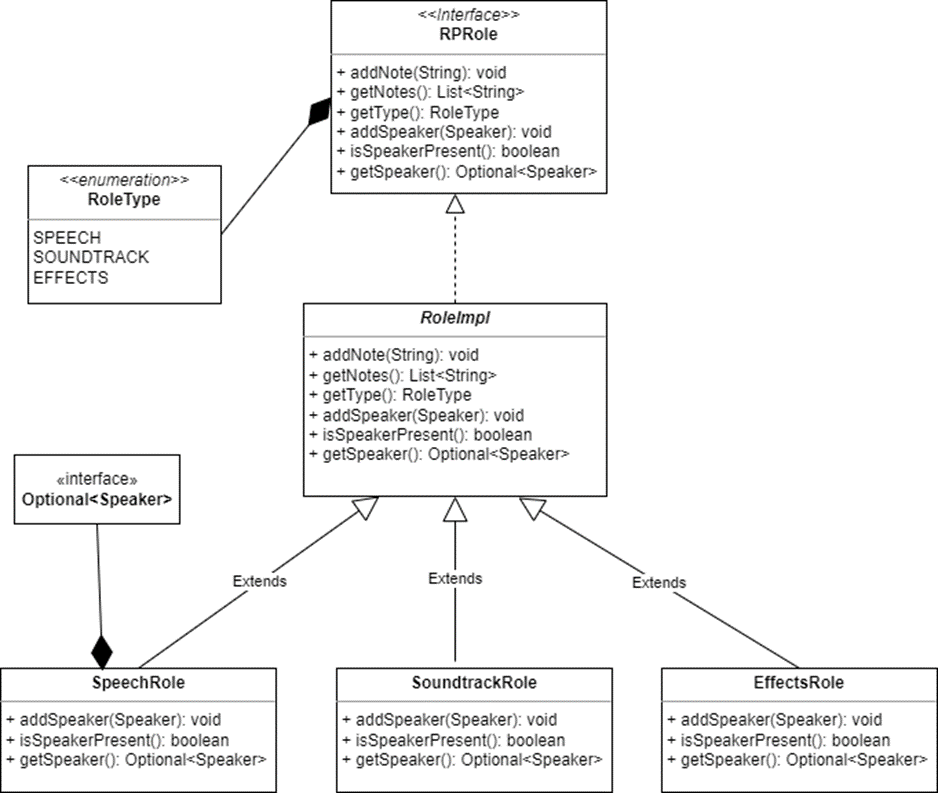
\includegraphics[width=\textwidth,scale=1]{img/role.png}
\caption{UML rappresentante Template Method sulla classe astratta “RoleImpl”.}
\end{figure}

\subsubsection{Progetto con comportamento comune anche con tipologie differenti}
Un altro elemento con una situazione simile è “RPProject”, l’entità che rappresenta l’intero progetto. Un RPProject può essere di diverse tipologie, ma questa volta la scelta è quella di rappresentarlo soltanto attraverso interfaccia più implementazione concreta, e non tramite Template Method. Questo perché non cambia comportamento a seconda della tipologia, ma è soltanto necessario conoscere la tipologia alla quale appartiene. Così si spiega la scelta di non utilizzare il pattern.

\subsubsection{Composizione tra timeline e tante section}
Gli ultimi due elementi portati dal basso all’alto livello sono “RPSection” e “RPTimeline”. In questo caso il problema è rappresentato dal fatto che una RPTimeline è costituita da più RPSection, che però non si possono sovrapporre in termini di tempo. La soluzione adottata consiste nel realizzare una composizione (i.e. una RPTimeline si compone di più RPSection), messa in atto attraverso una Map (struttura dati messa a disposizione dal package java.util), che mappa una RPSection alla sua durata. In questo modo è possibile effettuare, internamente a RPTimeline, controlli per evitare che le sue sezioni si possano sovrapporre.

\begin{figure}[h]
\centering{}
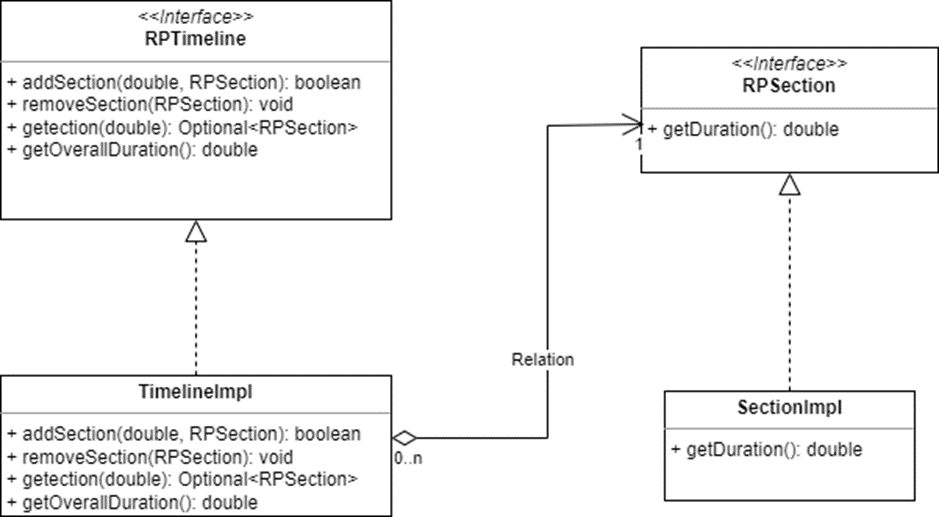
\includegraphics[width=\textwidth,scale=1]{img/timeline.png}
\caption{UML rappresentante Timeline che si compone di più RPSection.}
\end{figure}

\subsubsection{Molteplici costruzioni di speaker}
Una figura “esterna” alla DAW è quella di uno speaker, cioè quell’entità che può essere associata ad un RPRole di tipo Speech. La creazione di queste entità avviene per mezzo del relativo costruttore, ma per semplificare il procedimento, è stato realizzato un opportuno builder, tramite classe innestata all’interno di uno spekaer. In questo modo si ritiene più semplice la creazione di un oggetto di questo tipo, che secondo le stime potrà avvenire piuttosto di frequente.

\begin{figure}[h]
\centering{}
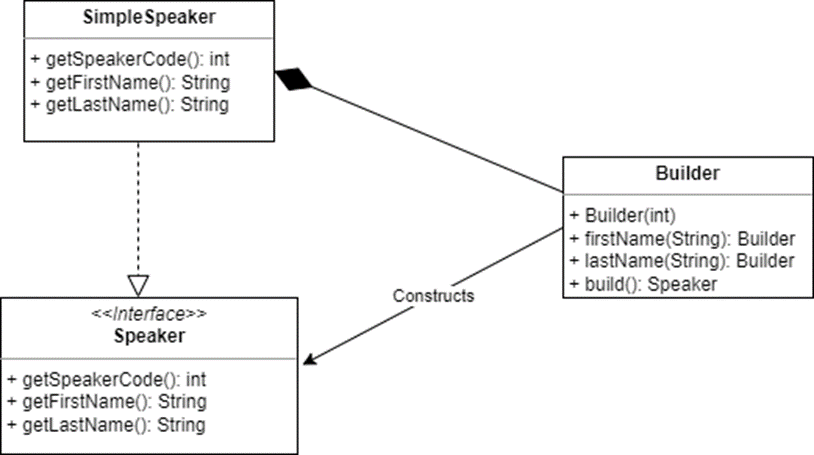
\includegraphics[width=\textwidth,scale=1]{img/speaker.png}
\caption{UML rappresentante Speaker e builder di speaker.}
\end{figure}

\subsubsection{Costruzione di una singola rubrica}
In seguito si è resa necessaria la creazione di una rubrica di speaker (“SpeakerRubric”), in modo che se lo stesso speaker debba partecipare ad un nuovo progetto, non si debbano inserire nuovamente i suoi dati, ma che questi li si abbiano già a disposizione. La rubrica è quindi composta da tanti speaker. In questo caso si è deciso di non usufruire di pattern creazionali, in quanto la rubrica va creata una tantum, e farlo attraverso pattern costituirebbe l’inserimento di un livello di complessità maggiore. Si sceglie quindi la strada più semplice, cioè la creazione della rubrica tramite costruttore vuoto.

\begin{figure}[h]
\centering{}
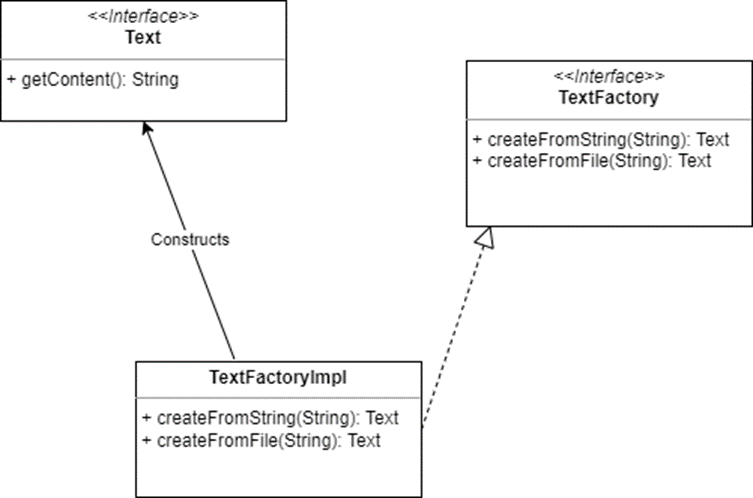
\includegraphics[width=\textwidth,scale=1]{img/text.png}
\caption{UML rappresentante Factory Method su Text.}
\end{figure}

\subsubsection{Costruzione di un elevato numero di testi}
Discorso completamente diverso è invece quello che riguarda l’ultima entità, costituita dal testo. In questo caso si prevede che spesso ci sarà necessità di associare un testo ad una RPPart di tipo Speech, che costituiranno la maggior parte dei progetti realizzati tramite l’applicativo. 

In questo caso costruire testi tramite costruttore risulterebbe poco pratico, poco riutilizzabile e piuttosto complesso, data anche la necessità di generare testo a partire da sorgenti diverse. Questa analisi mi ha portato quindi a fare ricorso ad un pattern creazionale, ed in particolare al Factory Method. In questo modo sono riuscito a separare quindi il concetto di testo nel senso stretto dalla sua creazione, ottenendo codice meglio organizzato e più facilmente leggibile. In questo modo in più, l’interfaccia del Factory Method semplifica l’aggiunta di nuove modalità di creazione in caso di future necessità. 

All’interno della famiglia delle Factories si è scelto proprio questo pattern in quanto fosse il più adeguato a realizzare la mia necessità: ho escluso Abstact Factory in quanto gli oggetti creati devono essere indipendenti, mentre Static Factory e Simple Factory avrebbero garantito meno estensibilità e più rigidità nel modificare il codice ed infine minor leggibilità.

\subsection{Luca Pasini}
\subsubsection{Manager}
La seguente parte di model serve ad unire le diverse componenti del software create dagli altri componenti del gruppo. Per fare ciò è stata creata una “centralina” che prendesse tutti gli elementi del programma e li unisse in strutture dati. 

La classe designata è il Manager che, oltre a salvare i dati, funge da finestra di accesso al software, fornendo i metodi necessari per interagire con il resto del programma. Il Manager inoltre prende decisioni per l’utente, come quella di raggruppare i canali che vengono creati. I gruppi sono canali “invisibili” all’utente che sono collegati al master. Tutti i canali creati dall’utente fanno parte di un gruppo quindi il loro output è collegato al gruppo e non direttamente al master.

I gruppi sono speaker, soundtrack ed effects. Il gruppo soundtrack ha un effetto di sidechaining al gruppo speaker (vedi sezione su RPEffect per saperne di più) mentre il gruppo effects è scollegato dagli altri due. In una prima implementazione all’utente era possibile scambiare elementi fra i gruppi, crearne di nuovi e anche avere canali in nessun gruppo, tuttavia è stata scartata in favore di una più semplice implementazione che comprende solo i gruppi sopra citati e che impedisce lo spostamento e la rimozione dai gruppi; in una futura implementazione è pianificato di aggiungere queste funzionalità. Il Manager si occupa anche della creazione e gestione di Clip e Sezioni. Le Clip vengono create specificando anche il canale a cui appartengono, il loro tempo di inizio all’interno di suddetto canale e la loro durata dipendente anche dalla presenza o assenza di contenuto. Alle Clip è possibile rimuovere o aggiungere contenuto dopo la creazione ed è inoltre possibile muoverle all’interno del canale, alterarne la durata e anche “splittarle”. Il Manager tiene inoltre conto della durata complessiva della timeline, con una durata minima di 10 minuti e che viene aggiornata dinamicamente all’aggiunta e alla modifica delle Clip. Infine il Manager si occupa anche della creazione di Sezioni e Rubrica, che aiutano l’utente nella gestione di un progetto. Per semplificare il compito del manager sono state create le classi RPClipLinker e RPChannelLinker che si occupano del collegamento fra alto e basso livello.

\begin{figure}[H]
\centering{}
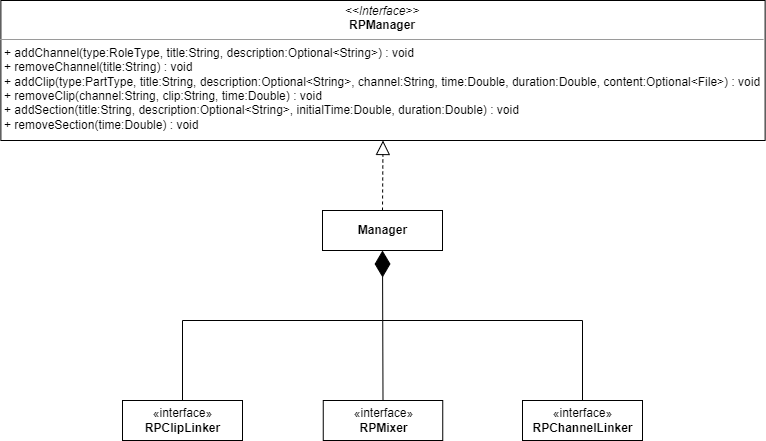
\includegraphics[width=\textwidth]{img/manager.png}
\caption{UML rappresentante Manager e le interfacce da esso utilizzate.}
\end{figure}

\subsubsection{Mixer}
Il Mixer è la classe utilizzata dal Manager per creari canali e gestire i collegamenti coi gruppi e con il master. Il Mixer utilizza una ChannelFactory per creare i canali e poi effettua il collegamento con il canale master creato e collegato all'Audio Context all’istanziazione della classe. Il Mixer inoltre include i metodi per collegare canali ad un gruppo.

\begin{figure}[H]
\centering{}
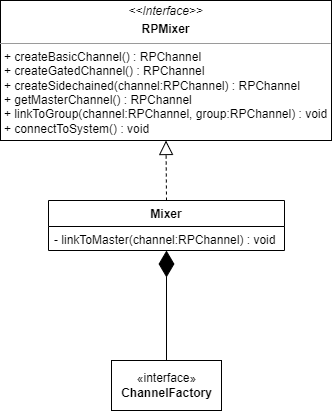
\includegraphics[scale=0.8]{img/mixer.png}
\caption{UML che illustra l'uso di Channel Factory da parte del Mixer.}
\end{figure}

\subsubsection{Channel Linker}
Il compito del Channel Linker è quello di collegare le varie parti che compongono un canale. Un canale è modellato da un RPRole che lo rappresenta ad alto livello, un RPChannel che lo rappresenta a basso livello ed un RPTapeChannel che è il “contenitore” delle Clip del canale. La struttura dati scelta per assecondare questo design è una mappa in cui le chiavi sono gli RPRole mentre i valori sono coppie di RPChannel e RPTapeChannel. Questo rende gli RPRole univoci ed identificabili dal titolo. La scelta di RPRole come chiave è stata fatta perché non è possibile garantire l’univocità di RPChannel e RPTapeChannel mentre per RPRole ciò è assicurato dalla presenza del titolo.

\begin{figure}[H]
\centering{}
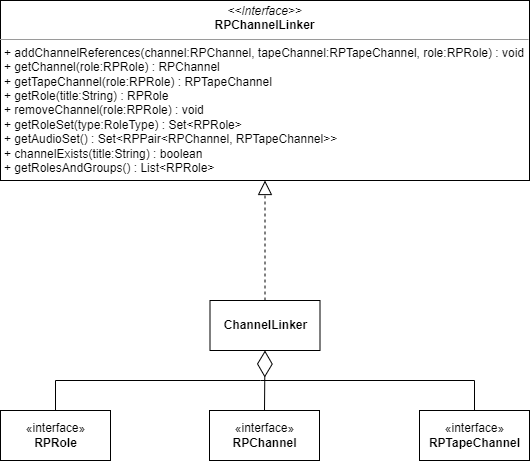
\includegraphics[width=\textwidth]{img/channelLinker.png}
\caption{UML che mostra quali dipendenze possiede ChannelLinker.}
\end{figure}

\subsubsection{Clip Linker}
Il compito del Clip Linker è quello di collegare la parte ad alto livello e quella a basso livello delle Clip. Come nel caso del channel linker la struttura dati scelta è una mappa con chiavi RPPart, identificati dal loro titolo, e con valori RPClip. Per problemi di implementazione abbiamo successivamente scelto di aggiungere un campo titolo anche nelle RPClip, identico al titolo della rispettiva RPPart, così da rendere possibile ottenere una RPPart a partire da una RPClip, creando così un associazione 1:1 fra RPClip e RPPart.

\begin{figure}[H]
\centering{}
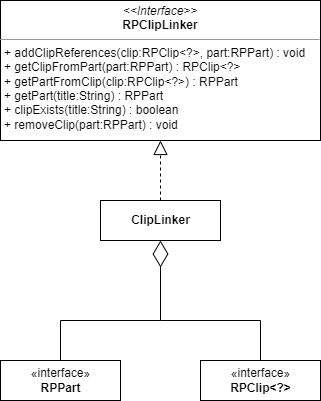
\includegraphics[scale=0.75]{img/clipLinker.png}
\caption{UML che mostra quali dipendenze possiede ClipLinker.}
\end{figure}

\subsection{Giacomo Sirri}
\subsubsection{RPChannel}
Questa parte di sviluppo del software si è focalizzata principalmente sulla implementazione dei canali audio. Come già accennato nell’analisi del dominio, per canale si intende il mezzo di comunicazione tra sorgenti audio e mixer. Ogni canale deve quindi essere dotato di un ingresso ed un’uscita. 

Per comprendere al meglio la sua funzione, si può pensare al canale audio come all’equivalente di un tubo in un sistema idraulico. Così come i vari condotti sono strutturalmente uguali e si distinguono esclusivamente per la loro funzione, allo stesso modo anche i canali non presentano differenze a livello di implementazione e vengono differenziati solo grazie al tipo. Sono presenti 3 tipi di canale: Audio, Return e Master, già introdotti nel glossario dei termini.
Il contenuto del canale master è quello che viene effettivamente riprodotto e quindi ad esso devono confluire gli output degli altri canali. 

Si noti che, per quanto detto prima, i canali di ritorno e il canale master devono avere gli stessi metodi e campi dei canali audio standard, differenziandosi da questi ultimi solo per il tipo. Ciò ha portato ad escludere la modellazione con Template Method inizialmente considerata. Il canale è rappresentato ad alto livello dall’interfaccia RPChannel e a livello implementativo dalla classe BasicChannel. 

Si giunge quindi allo schema UML in figura:

\begin{figure}[H]
\centering{}
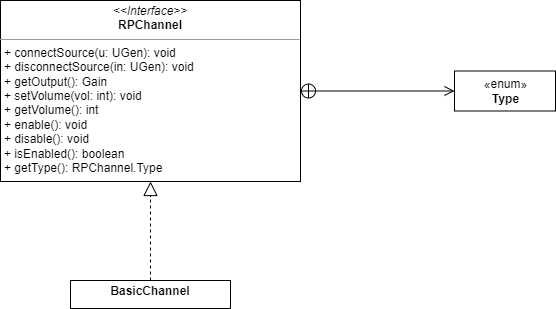
\includegraphics[width=\textwidth,scale=1]{img/channel.png}
\caption{UML di RPChannel e BasicChannel.}
\end{figure}

\subsubsection{Processing Unit}
Processare l’audio importato o registrato in un canale è una delle feature più importanti che le DAW commerciali mettono a disposizione degli utenti. Per questo motivo, sebbene il concetto di canale presentato nell’analisi del dominio venga retto già da questa prima implementazione, si è deciso di dotare i canali della possibilità di avere una processing unit. Per processing unit si intende una sequenza di effetti audio che elaborano e modificano il segnale in ingresso, producendo un output che dipende dal tipo e dall’ordine degli effetti. 
L’ingresso della processing unit viene collegato all’ingresso del canale, mentre l’uscita viene collegata all’uscita del canale (quest’ultima in realtà è preceduta da altri device opzionali di manipolazione audio che gestiscono volume, muteness e panning del canale).

Per evitare ambiguità tra un canale dotato di processing unit vuota e un canale senza processing unit, si è optato per imporre la presenza di almeno un effetto all’interno di una processing unit, dal momento della sua creazione a quello della sua eventuale rimozione dal canale di appartenenza.
La scelta si è basata sul fatto che la presenza di una processing unit all’interno di un canale è meramente opzionale, in quanto il concetto di canale è già modellato senza la necessità di inserirvi una processing unit.

Questa feature fa sì che i canali possano essere distinti non più solo dal tipo, bensì anche dalla processing unit di cui sono dotati e si può addirittura pensare di mettere a disposizione dell’utente delle configurazioni ready-to-use di canali. Ciò risulta particolarmente utile per differenziare già dalla creazione i canali riservati agli speaker da quelli destinati a contenuti musicali.
Per automatizzare la creazione dei canali preimpostati, il mixer utilizza i metodi dell’interfaccia ChannelFactory, la quale aderisce al pattern Factory Method. In sostanza, i metodi della factory ritornano canali che si distinguono per il loro tipo e/o processing unit. Oltre ai canali di ritorno e al master, la factory fornisce metodi per creare canali basic, gated e sidechained. I primi si distinguono per l’assenza della processing unit, i secondi sono quelli più indicati per il processing della voce, mentre gli ultimi sono pensati per i contenuti musicali, come ad esempio la sigla di un podcast (si veda la sezione su RPEffect per saperne di più).

Per rendere il design ancora più facilmente aggiornabile ed espandibile, la factory si appoggia su ProcessingUnitBuilder, un’interfaccia Builder dotata dei metodi necessari ad aggiungere effetti alla processing unit in costruzione. In questo modo, se si decidesse di modificare l’implementazione a basso livello degli effetti, la factory non subirebbe cambiamenti, poiché a cambiare sarebbe l’implementazione dei metodi del builder.
Schematizzando quanto detto si ottiene l’UML sottostante:

\begin{figure}[H]
\centering{}
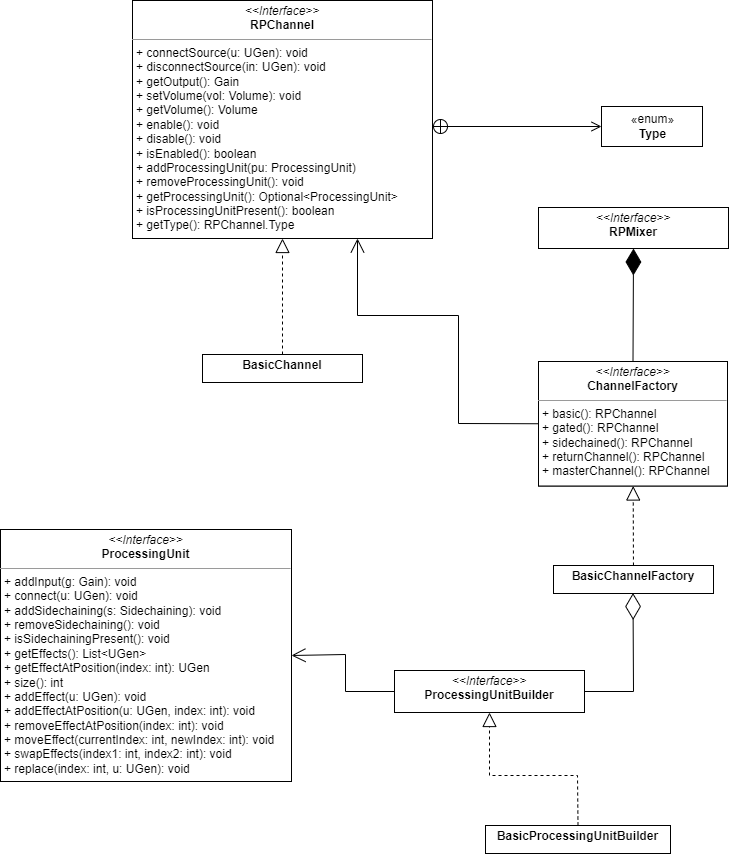
\includegraphics[width=\textwidth]{img/processingUnit.png}
\caption{UML che mostra l'interazione tra ProcessingUnit e RPChannel, con pattern FactoryMethod e Builder.}
\end{figure}

\subsubsection{RPEffect}
E’ necessario ora modellare tutte quelle entità che fino ad ora sono state menzionate con il generico termine “effetti”. Come già detto, gli effetti elaborano un segnale audio, restituendo in output una versione modificata del segnale in ingresso. 

Si rende quindi indispensabile lavorare a basso livello su buffer contenenti i dati che rappresentano digitalmente l’audio. Implementare i metodi per il processing del segnale (uno per ogni effetto) sarebbe stato un compito molto gravoso, nonché decisamente inadeguato a future estensioni.
Si è pertanto cercata una libreria che fornisse una API per la gestione dell’audio a basso livello. La scelta è ricaduta su Beads, una libreria open-source “for programming audio in Java for musical and other creative sound applications”. 

L’elemento centrale della libreria è la classe astratta UGen (Unit Generator), che modella “subroutines that take input, do something to it, then send the results out of their outputs”.
Un esempio fondamentale di sottoclasse di UGen è la classe Gain, che serve a controllare il volume di un segnale audio. A livello implementativo, ogni qualvolta è necessario un elemento per rappresentare l’ingresso o l’uscita di una parte del sistema (canale, processing unit, effetti), tale posizione viene occupata da un oggetto di tipo Gain.
Gli UGen possono avere più canali di input e output. Il termine canale non deve trarre in inganno: non si sta qui parlando del canale audio modellato da RPChannel, bensì di una porta attraverso la quale passa un segnale. Un Gain, ad esempio, può essere dotato di più canali di ingresso, in modo tale da poter ricevere input da due sorgenti sonore diverse.

Per quanto riguarda il design di questa porzione di model, la prima scelta fondamentale è stata quella di fattorizzare tutte le operazioni in comune tra i vari effetti nella classe astratta RPEffect. Le implementazioni concrete di tale classe possiedono tutte un Gain di entrata e uno di uscita e si distinguono per come processano il segnale in ingresso: serve quindi un metodo astratto, che sarà compito delle sottoclassi stesse implementare, il quale specifichi come ottenere l’output a partire da un certo input. L’unico metodo astratto della classe UGen (calculateBuffer) ha uno scopo analogo, quindi risulta naturale che RPEffect estenda UGen. 

La modellazione prevede in sostanza che ogni RPEffect racchiuda al suo interno (wrapping) una classe di Beads che sia sottoclasse di UGen e che fornisca un’implementazione di calculateBuffer in grado di facilitare il calcolo dell’output dell’effetto stesso. Si noti che in questo modo l’elemento di libreria utilizzato è perfettamente incapsulato all’interno dell’effetto, rendendone l’uso trasparente alle classe esterne. Qualora si decidesse di cambiare la classe di libreria “wrappata” dall’effetto, cosa tra l’altro verificatasi con frequenza durante lo sviluppo, l’ambiente software circostante non ne risentirebbe minimamente. 

L’indubbia pecca di questo design è che alla sua sommità si trovi una classe astratta: per questo motivo, i metodi di carattere generale individuati per gli effetti sono andati a confluire nell’interfaccia AudioElement, la quale modella un generico elemento audio con un ingresso, un’uscita e degli eventuali parametri. Infatti, tra i metodi non astratti che ad una prima implementazione erano stati dichiarati in RPEffect, particolarmente meritevoli di menzione sono i metodi (getter e setter) che agiscono sui parametri. I parametri sono i valori sulla base dei quali un elemento audio processa il suono. Ovviamente, essi sono specifici per un singolo effetto, o tuttalpiù per una famiglia di effetti. 

Questa modifica ha anche il pregio che se si volesse in futuro estendere una classe di libreria, per esempio Gain, essa potrebbe sia estendere la relativa classe di libreria che anche implementare l’interfaccia AudioElement, semplificando notevolmente l’integrazione con il resto del software.
 
Entriamo ora nel dettaglio delle implementazioni di RPEffect.
Gli effetti implementati in questo software sono: compressore (con variante sidechaining), limiter, high pass filter, low pass filter, gate e riverbero. 
Al di là del sidechaining, tutti questi effetti sono modellati da classi che o estendono direttamente RPEffect, oppure estendono una classe che a sua volta estende RPEffect. Il design che si è scelto di implementare raggruppa infatti gli effetti simili in categorie, rappresentate da una classe astratta che si frappone tra essi ed RPEffect. 

Una caratteristica importante di questa modellazione è che gli effetti che fanno parte di una categoria non implementano calculateBuffer, poiché esso viene fattorizzato nella classe astratta che modella la categoria stessa. In altre parole, due effetti sono della stessa categoria se producono il proprio output tramite lo stesso algoritmo. Ciò che cambia tra di essi può essere ad esempio il valore di default di un certo parametro, oppure quale uscita dell’output viene utilizzata (in caso di effetti con più canali di uscita).

Si descrivono ora brevemente i vari effetti:
\begin{itemize}
    \item Compressore e limiter: attenuano (eliminano nel caso del limiter) le porzioni del segnale in ingresso per le quali l’ampiezza del segnale supera una certa soglia. Compongono la categoria detta dinamica del suono, modellata dalla classe astratta Dynamics.
    \item Riverbero: simula l’omonimo fenomeno fisico (anche detto eco), che si ottiene ad esempio battendo le mani in una stanza vuota.
    \item Low e high pass filter: impediscono il passaggio di tutte le frequenze che si trovano al di sopra (sotto) di una certa soglia. Compongono la categoria detta equalizzazione, modellata dalla classe astratta Equalization.
    \item Gate: attenua o elimina le porzioni del segnale in ingresso per le quali l’ampiezza del segnale è inferiore ad un certa soglia.
\end{itemize}
Un discorso a parte va fatto per il sidechaining. Nell’ambito del processing audio, un compressore si dice sidechained quando la sorgente da esso utilizzata per calcolare il livello di compressione è esterna, cioè non coincide con la sorgente sulla quale il compressore agisce. La tecnica del sidechaining è molto usata nei podcast. infatti, è piuttosto frequente che la sigla di un podcast cominci prima che il conduttore abbia finito l’introduzione; per evitare la sovrapposizione tra musica e voce, nel canale in cui si trova la sigla viene posto un compressore sidechained verso la voce, così il volume della sigla venga attenuato fino a quando il conduttore non finisce di parlare. 

Per quanto il sidechaining sia un sottotipo di RPEffect, in particolare della categoria di dinamica, esso presenta qualche peculiarità. Un effetto di tipo sidechaining, infatti, non può essere posizionato in un punto qualsiasi della processing unit come accade per gli altri effetti, bensì solo in prima posizione (cioè riceve l’input direttamente dal canale). In altre parole, una processing unit o è sidechained verso un’altra sorgente, e quindi ha in prima posizione un effetto di tipo sidechaining, oppure non lo è. Per poter far rispettare questi vincoli lato processing unit, si è pensato di introdurre la tag interface Sidechaining. Il fatto che la classe che rappresenta il sidechaining implementi tale interfaccia fa sì che il sidechaining abbia un tratto distintivo rispetto agli altri effetti, proprio come nella realtà modellata.

\begin{figure}[H]
\centering{}
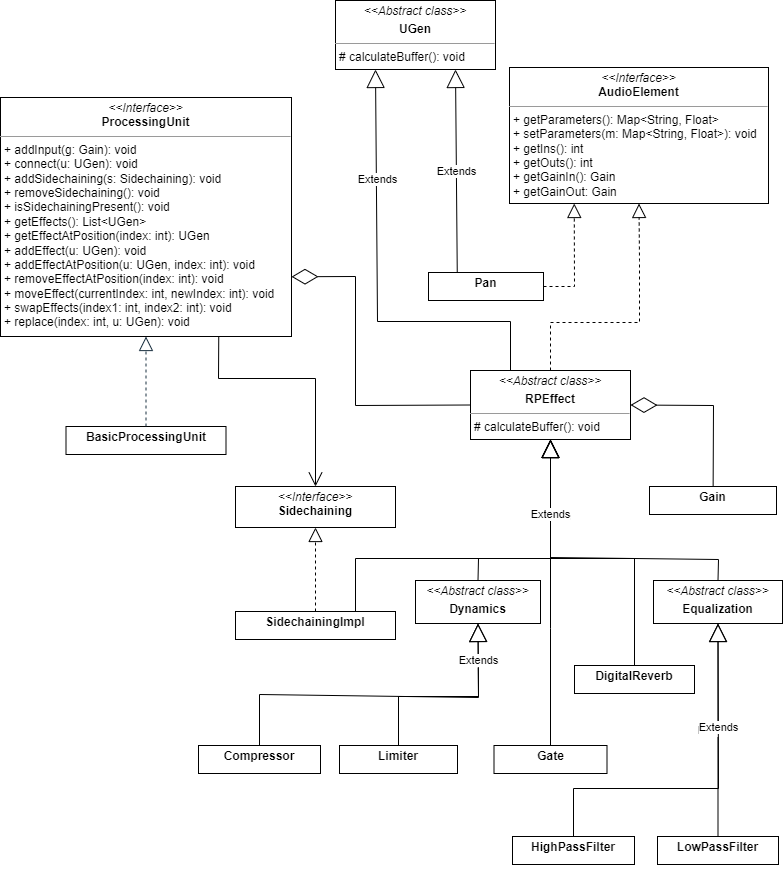
\includegraphics[width=\textwidth]{img/effect.png}
\caption{Rappresentazione della gerarchia degli effetti, a partire da AudioElement fino ad arrivare alle implementazioni degli effetti.}
\end{figure}

\chapter{Sviluppo}
\section{Testing automatizzato}
Varie parti del software sono state sottoposte a testing automatizzato tramite la suite JUnit (versione 5).
In particolare sono state realizzate classi di testing per i seguenti componenti del modello:
\begin{itemize}
    \item Clip,
    \item Tape channel,
    \item Clock,
    \item ClipPlayerNotifier,
    \item Channel,
    \item Processing unit,
    \item Manager,
    \item Planning.
\end{itemize}
Sono inoltre state realizzate classi di testing automatizzato per lo storing e la serializzazione.
Non è invece stato possibile testare in modo automatizzato alcune classi dell’Engine, in quanto sarebbe stato necessario avere dei progetti realizzati in Resplan su cui testarne il comportamento. 
Per lo stesso motivo, il ClipPlayerNotifier ha un test automatizzato che prima di essere eseguito deve creare una PlayersMap su cui eseguire il test.
Per le classi su cui non è stato possibile eseguire test automatizzati è stato necessario effettuare vari test manuali.
L’applicazione è stata testata su diversi sistemi operativi (Windows, OSX, Linux) e su schermi di diverse risoluzioni (Full HD, 2K, 4K).
Alcuni problemi emersi riguardano la scelta del dispositivo di input audio. Non sempre il dispositivo di default per l’input audio rilevato dalla Java Sound API si rivela essere funzionante. Purtroppo non è stata trovata soluzione al problema, se non quella di forzare dal sistema operativo l’utilizzo del dispositivo desiderato come dispositivo di default. Tuttavia anche questa metodologia non sempre si rivela funzionante.

\section{Metodologia di lavoro}
La metodologia di lavoro con cui si è affrontato lo sviluppo di nuove features è stata la seguente: per ogni nuova componente del software da sviluppare è stato analizzato nei dettagli il comportamento atteso.
In seguito è stata creata una prima versione della nuova componente cercando di riutilizzare il più possibile il codice già scritto.
Per ogni tentativo venivano eseguiti test per verificare il corretto funzionamento dell’entità creata. 
Una volta ottenuta una prima versione funzionante sono state eseguite rifattorizzazioni per migliorare la qualità del codice scritto e suddividere le singole responsabilità tra oggetti diversi. Quando è stata individuata la possibilità di utilizzare qualche pattern di design questo è stato applicato.
Se emergevano dipendenze tra le varie classi si cercava di scioglierle, così come, per ogni classe, si è cercato di prevedere quali potessero essere le possibili evoluzioni future in modo da riadattare il codice per renderlo facilmente estendibile in futuro, senza dover modificare quello già scritto.
Infine l’ultimo step rimaneva sempre quello di verificare il comportamento delle componenti sviluppate nei casi più complicati.

Per coordinare il lavoro del gruppo sono stati divisi i compiti in modo da assegnare alla stessa persona lo sviluppo di classi riguardanti concetti simili. Nello specifico, a Menghi sono state assegnate le classi di planning, ad Antonini quelle che gestiscono le clip audio e gli elementi necessari a registrarle e riprodurle, Sirri si è occupato delle componenti audio a basso livello e Pasini ha gestito la logica generale dell'applicazione.

Dopo di che, è stato necessario definire le interfacce principali necessarie all’interazione tra le diverse parti dell’applicazione.
In una prima fase è stato necessario confrontarsi per spiegare e definire alcuni concetti riguardanti la produzione audio e le relative tecnologie. Infatti, non tutti i membri del gruppo possedevano conoscenze approfondite del dominio applicativo in questione. 
Una volta iniziata la fase individuale di sviluppo del codice, non sono comunque mancate interazioni tra i membri del gruppo, utili a confrontarsi e aggiornarsi sui progressi e sulle difficoltà incontrate.

Git e GitHub sono stati strumenti fondamentali per unificare e organizzare il lavoro di ogni membro del gruppo. Per ogni feature da sviluppare, infatti, è stato creato un branch di sviluppo indipendente, nel quale il responsabile ha a termine il proprio lavoro per poi unificarlo con il codice degli altri. Solo nell'ultima fase di sviluppo si è utilizzato un unico branch, in modo tale che tutti i componenti avessero a disposizione la stessa implementazione delle classi comuni di view e controller.

\subsection{Responsabilità}
\subsubsection{Alessandro Antonini}

\begin{center}
\begin{longtable}{| m{22.5em} | m{2cm}| m{1cm} | m{2.7cm} |} 
 \hline
  \textbf{Nome} & \textbf{Tipologia} & \textbf{MVC} & \textbf{Collaboratori} \\ [0.5ex]
 \hline
 daw.core.clip & package & M & - \\ 
 \hline
 daw.engine & package & M & - \\
 \hline
 daw.utilities.MapToSet & class & M & - \\
 \hline
 daw.utilities.HashMapToSet & class & M & - \\
 \hline
 view.common.ChannelsView & class & V & - \\
\hline
 view.common.ChannelInfosView & class & V & - \\
\hline
view.common.ChannelContentView & class & V & - \\
\hline
view.common.ClipDragModality & class & V & - \\
\hline
view.common.MarkersPane & class & V & - \\
\hline
view.common.NumberFormatConverter & class & V & Luca Pasini \\
\hline
view.common.RegionHeightResizer & class & V & - \\
\hline
view.common.TimeAxisDragNavigator & class & V & - \\
\hline
view.common.TimeAxisSetter & class & V & - \\
\hline
view.common.Tool & class & V & - \\
\hline
view.common.ToolBarSetter & class & V & - \\
\hline
view.common.ToolChangeListener & class & V & - \\
\hline
view.common.ViewData & class & V & - \\
\hline
view.common.ViewDataImpl & class & V & - \\
\hline
view.edit & package & V & - \\
\hline
src/main/resources/view/EditView.fxml & FXML & V & - \\
\hline
src/main/resources/view/RecorderView.fxml & FXML & V & - \\
\hline
\end{longtable}
\end{center}
Il codice della classe RegionHeightResizer è stato preso da un thread di GitHub Gist ed è stato riadattato per essere utilizzato nella classe in questione:
\href{https://gist.github.com/andytill/4369729}{https://gist.github.com/andytill/4369729}

\subsubsection{Gabriele Menghi}
\begin{center}
\begin{longtable}{| m{22.5em} | m{2cm}| m{1cm} | m{2.7cm} |} 
 \hline
 \textbf{Nome} & \textbf{Tipologia} & \textbf{MVC} & \textbf{Collaboratori} \\ [0.5ex]
 \hline
  planning & package & M & - \\
 \hline
 view.effects & package & V & - \\
 \hline
view.effects.EffectsPane & class & V & Alessandro Antonini \\
\hline
 \end{longtable}
 \end{center}

\subsubsection{Luca Pasini}
\begin{center}
\begin{longtable}{| m{22.5em} | m{2cm}| m{1cm} | m{2.7cm} |} 
 \hline
   \textbf{Nome} & \textbf{Tipologia} & \textbf{MVC} & \textbf{Collaboratori} \\ [0.5ex] 
\hline
daw.core.mixer & package & M & - \\
\hline
daw.manager & package & M & - \\
\hline
resplan & package & C & - \\
\hline
controller.general.Controller & class & C & Giacomo Sirri \\
\hline
controller.general.ControllerImpl & class & C & Giacomo Sirri \\
\hline
view.common.AlertDispatcher & class & V & - \\
\hline
view.common.App & class & V & - \\
\hline
view.common.FilePicker & class & V & - \\
\hline
view.common.JsonFilePicker & class & V & - \\
\hline
view.common.TextFilePicker & class & V & - \\
\hline
view.common.WavFilePicker & class & V & - \\
\hline 
view.common.NumberFormatConverter & class & V & Alessandro Antonini \\
\hline
view.common.RecorderController & class & V & - \\
\hline
view.common.ResizeHelper & class & V & - \\
\hline
view.common.WindowBar & class & V & - \\
\hline
view.planning & package & V & Giacomo Sirri \\
\hline
src/main/resources/view/ExportView.fxml & FXML & V & - \\
\hline
src/main/resources/view/NewChannelWindow.fxml & FXML & V & - \\
\hline
src/main/resources/view/NewClipWindow.fxml & FXML & V & - \\
\hline
src/main/resources/view/NewSectionWidow.fxml & FXML & V & - \\
\hline
src/main/resources/view/PlanningView.fxml & FXML & V & - \\
\hline
src/main/resources/stylesheets/resplan.css & CSS & V & - \\
\hline
\end{longtable}
\end{center}
Il codice della classe ResizeHelper è stato preso e modificato da un thread di Stack Overflow:
\href{https://stackoverflow.com/questions/19455059/allow-user-to-resize-an-undecorated-stage}{https://stackoverflow.com/questions/19455059/allow-user-to-resize-an-undecorated-stage}

\subsubsection{Giacomo Sirri}
\begin{center}
\begin{longtable}{| m{22.5em} | m{2cm}| m{1cm} | m{2.7cm} |} 
 \hline
   \textbf{Nome} & \textbf{Tipologia} & \textbf{MVC} & \textbf{Collaboratori} \\ [0.5ex] 
 \hline
  daw.core.channel & package & M & - \\
  \hline
daw.core.audioprocessing & package & M & - \\
\hline
controller.storing & package & C & - \\
\hline
controller.storing.deserialization & package & C & - \\
\hline
controller.storing.serialization & package & C & - \\
\hline
controller.general.LoadingException & class & C & - \\
\hline
controller.general.DownloadingException & class & C & - \\
\hline
controller.general.ProjectDownloader & class & C & - \\
\hline
controller.general.ProjectDownloaderImpl & class & C & - \\
\hline
controller.general.ProjectLoader & class & C & - \\
\hline
controller.general.ProjectLoaderImpl & class & C & - \\
\hline
view.planning.ChannelDescriptionEditorController & class & V & - \\
\hline
view.planning.ClipDescriptionEditorController & class & V & - \\
\hline
view.planning.ClipTextEditorController & class & V & - \\
\hline
view.planning.RubricController & class & V & - \\
\hline
view.planning.TextEditorController & class & V & Luca Pasini \\
\hline
src/main/resources/view/TextEditorView.fxml & FXML & V & Luca Pasini \\
\hline
src/main/resources/view/RubricView.fxml & FXML & V & - \\
\hline
\end{longtable}
\end{center}
Il codice di RubricView.fxml è stato tratto in gran parte da un tutorial di Oracle:
\href{https://docs.oracle.com/javase/8/javafx/fxml-tutorial/fxml\_tutorial\_intermediate.htm}{https://docs.oracle.com/javase/8/javafx/fxml-tutorial/fxml\_tutorial\_intermediate.htm}

\section{Note di sviluppo}
\subsection{Scelta della libreria audio}
La scelta della libreria audio è stata fondamentale per lo sviluppo di Resplan.
Java mette a disposizione la Java Sound API, una libreria di basso livello che permette di controllare l’Input/Output audio e MIDI di sistema. 
Tuttavia analizzando meglio la libreria sono emerse alcune limitazioni tra cui:
\begin{itemize}
    \item Impossibilità di scegliere quale canale di I/O dell’interfaccia audio utilizzare (la libreria permette di utilizzare solo quello impostato di default nel sistema operativo).
    \item La somma di varie sorgenti audio digitali in un unico stream audio non è implementata nella libreria.
    \item Non vengono fornite classi o metodi per processare l’audio.
\end{itemize}
Abbiamo quindi scelto di utilizzare una libreria audio di più alto livello: Beads.

Questa libreria si appoggia sulla Java Sound API, ma fornisce la possibilità di processare l’audio ed effettuarne il routing tramite catene di dispositivi chiamati UGen.
Questi possono essere sia generatori di audio (oscillatori, lettori di file audio, ecc…), che effetti che processano l’audio che vi passa all’interno.
Gli UGen funzionano scrivendo e leggendo dati da un buffer audio (array di byte contenenti i sample dell’audio digitale). Questo buffer viene elaborato in tempo reale e passato di UGen in UGen fino ad arrivare all’output dell’AudioContext. Quest’ultimo prende il buffer in uscita dall’ultimo UGen della catena e lo passa alla Java Sound API, la quale lo riproduce tramite l’output audio di sistema.

Purtroppo, essendo imposta dalla Java Sound API, rimane la limitazione di non poter scegliere il canale da utilizzare per l’I/O Audio. Tuttavia, Beads permette la somma dell’audio di diverse sorgenti e fornisce UGen già implementati per il processing dell’audio, features che altrimenti sarebbero dovute essere sviluppate da zero, formulando algoritmi di basso livello per modificare il buffer audio nel modo desiderato.

\subsection{JavaFX, FXML}
Per lo sviluppo della parte di View è stata utilizzata la libreria esterna JavaFX.
Sono state realizzate alcune parti in linguaggio FXML, mentre altre componenti di view sono state scritte direttamente in linguaggio Java.
\subsection{Gradle}
È stato utilizzato Gradle come Build Automation Tool per gestire le dipendenze delle librerie (JavaFX, Beads, ed altre) e per creare il JAR eseguibile.

\subsection{Features avanzate}
\subsubsection{Alessandro Antonini}
Si riporta l’utilizzo delle seguenti features avanzate del linguaggio Java:
\begin{itemize}
    \item Sviluppo delle interfacce o classi generiche:
    \begin{itemize}
        \item MapToSet\begin{math}<\end{math}X,Y\begin{math}>\end{math}
        \item HashMapToSet\begin{math}<\end{math}X,Y\begin{math}>\end{math}
        \item RPClip\begin{math}<\end{math}X\begin{math}>\end{math}
    \end{itemize}
    \item Utilizzo degli stream e delle lambda in diverse classi quali:
    \begin{itemize}
        \item TapeChannel
        \item PlayersMapBuilder
        \item ClipPlayerNotifier
        \item Action Listeners della view
    \end{itemize}
    \item Utilizzo di Optional in: 
    \begin{itemize}
        \item PlayersMapBuilder
        \item Engine
        \item ViewDataImpl
    \end{itemize}
    \item Concorrenza e multithread:
    \begin{itemize}
        \item Conductor
    \end{itemize}
\end{itemize}

\subsubsection{Gabriele Menghi}
Features avanzate utilizzate:
\begin{itemize}
    \item Lambda expressions nelle classi:
    \begin{itemize}
        \item TextFactoryImpl
        \item TimelineImpl
        \item molte delle classi del package “view.effects”
    \end{itemize}
    \item Method reference nelle classi:
    \begin{itemize}
        \item SimpleSpeakerRubric
        \item ContinuousKnobPane
        \item JerkyKnobPane
    \end{itemize}   
    \item Reflection nelle classi:
    \begin{itemize}
        \item EffectsPane
    \end{itemize}
    \item Interfacce funzionali:
    \begin{itemize}
        \item Text
    \end{itemize}
    \item Stream nelle classi:
    \begin{itemize}
        \item SimpleSpeakerRubric
        \item TimelineImpl
    \end{itemize}
    \item Optional nella maggior parte delle classi costituenti il package “planning”.
    \item Utilizzo di properties e listeners nelle classi:
    \begin{itemize}
        \item ContinuousKnobPane
        \item JerkyKnobPane
        \item EffectsPane
    \end{itemize}
    \item Uso della libreria JavaFX nelle classi del package. “view.effects”
\end{itemize}
Nella mia parte di progetto, di librerie non approfondite a lezione, ho utilizzato prevalentemente JavaFX, per la realizzazione della parte grafica. È stata poi utilizzata la classe “URL” del package java.net, utilizzata come parametri del metodo “setLocation()” della classe “FXMLLoader”, utilizzato per identificare le risorse da utilizzare sempre nell’interfaccia.
Un algoritmo degno di nota, implementato nel metodo “getOverallDuration()” nella classe “TimelineImpl”, che calcola la durata totale della timeline analizzando tutte le sezioni in essa presenti, prendendo quella con tempo di inizio maggiore e domandandone la relativa durata, ottenendo così appunto la durata totale.

\subsubsection{Luca Pasini}
Si riporta l’utilizzo delle seguenti funzioni avanzate:
\begin{itemize}
    \item Utilizzo di lambda e stream nelle seguenti classi:
    \begin{itemize}
        \item ClipLinker
        \item ChannelLinker
        \item Manager
        \item ControllerImpl
    \end{itemize}
    \item Method reference:
    \begin{itemize}
        \item RPManager
        \item Controller
    \end{itemize}
    \item Concorrenza e ScheduledExcutor:
    \begin{itemize}
        \item ExportViewController
    \end{itemize}
    \item Utilizzo di properties e listeners:
    \begin{itemize}
        \item WindowBar
        \item ResizeHelper
    \end{itemize}
\end{itemize}
\subsubsection{Giacomo Sirri}
Si riporta l’utilizzo delle seguenti funzionalità avanzate del linguaggio Java:
\begin{itemize}
    \item Utilizzo di lambda e stream in:
    \begin{itemize}
        \item ControllerImpl
    \end{itemize}
    \item Utilizzo di Optional in:
    \begin{itemize}
        \item BasicChannel
    \end{itemize}
    \item Utilizzo di reflection nei test sulla processing unit.
    \item Tag interface (Sidechaining).
    \item Utilizzo della libreria open-source Jackson per la serializzazione e deserializzazione del progetto in file JSON. Jackson è un processore JSON ad alte prestazioni che permette di serializzare e deserializzare il codice in maniera semi-automatizzata. Si era inizialmente considerato l’utilizzo di Gson, ma si è poi optato per Jackson in virtù della sua maggior facilità di utilizzo.
    \item Utilizzo della libreria open-source Beads per l’implementazione degli effetti.
\end{itemize}

\chapter{Commenti finali}
\section{Autovalutazione e lavori futuri}
\subsection{Alessandro Antonini}
La realizzazione di Resplan è stata la mia prima esperienza di sviluppo di un'applicazione completa. All’interno del gruppo ho condiviso la mia forte passione per la musica e per la produzione audio ed ho trasmesso agli altri componenti i concetti di dominio necessari per poter sviluppare il modello dell’applicazione.
Il lavoro in team è stato svolto in maniera efficiente e collaborativa, anche se le tempistiche si sono rivelate brevi per realizzare tutte le features che avevamo pianificato di sviluppare. In particolare sarebbe stato utile avere più tempo a disposizione per risolvere alcuni “bug” della view e collegare tutte le features sviluppate alla view e al controller.
Avrei voluto anche approfondire alcuni aspetti utili a perfezionare il nostro progetto come per esempio alcune parti di view, tra cui gli analizzatori dell’audio in tempo reale (oscillatori, analizzatori di spettro e vu-meters) e la visualizzazione della waveform dei file audio delle clip. Inoltre mi sarebbe piaciuto studiare gli algoritmi per manipolare e processare l’audio digitale.

Tra le varie problematiche sorte durante la realizzazione del progetto vorrei evidenziare quella delle limitazioni imposte dalle librerie audio. L’impossibilità di poter scegliere il canale di input/output dell’interfaccia audio non ha permesso di poter effettuare registrazioni contemporanee da sorgenti diverse su più canali, limitando l’usabilità dell’applicazione in un contesto professionale.
Sono comunque soddisfatto del lavoro svolto, in particolare per quanto riguarda il modello. 
Mi piacerebbe in futuro completare l’applicazione con tutte le features previste, magari dopo aver trovato una soluzione ai problemi imposti dalla libreria audio.

\subsection{Gabriele Menghi}
A mio parere i punti di forza della parte di software prodotta da me, sono la chiarezza del codice, la sua corretta organizzazione e l’uso degli adeguati pattern per rendere il tutto più comprensibile, ed anche estendibile. Un ulteriore punto di forza è la scelta efficace di nomi di metodi e campi. 

I punti di debolezza maggiori sono la scarsa complessità del codice scritto, scelta fatta però per favorire la chiarezza, e, soprattutto nella parte dell’interfaccia grafica, il fatto che in certi punti si hanno blocchi di codice confusionari, che sarebbero potuti essere scritti in maniera più ordinata stilisticamente parlando, anche se ho cercando di rispettare sempre le convenzioni.

Riguardo il mio ruolo all’interno del gruppo, prima di sottomettere la proposta di progetto abbiamo deciso come dividerci le parti di model; di comune accordo si è deciso che a me sarebbe spettata la parte di alto livello, in quanto ero colui che di audio aveva capito un po' meno dei quattro; in questo modo mi sarei dovuto concentrare meno sul capire i dettagli tecnici e più su quelli implementativi e del linguaggio. Riguardo alla grafica ho proposto poi di prendere la parte più ricca e complessa, in quanto già prima mi era toccata una parte più “leggera”. Parte che poi abbiamo deciso di dividere con Antonini, in quanto fin troppo complessa per essere svolta singolarmente. Non sono stato sicuramente l’elemento imprescindibile del gruppo, ma ho cercato di dare comunque il mio aiuto dall’inizio alla fine.

Infine, sono lasciate a sviluppi futuri le implementazioni del movimento del pannello di un effetto verso destra o verso sinistra (swap tra effetti) e l’aggiornamento in tempo reale dei vu-meter componenti alcuni effetti, indicanti la compressione corrente.

\subsection{Luca Pasini}
La realizzazione di questo progetto mi ha portato allo sviluppo di nuove competenze, tra cui il lavoro di gruppo e l’utilizzo di un DVCS.  Ho espanso inoltre le mie conoscenze del linguaggio java e della libreria JavaFX che ho usato molto per la creazione della View dandomi inoltre un infarinatura generale di CSS. 

Ritengo che il gruppo abbia lavorato bene nello sviluppo del progetto, per quanto probabilmente abbiamo preso un approccio complicato, decidendo di non partire da un'applicazione di base con poche funzionalità da espandere ma partendo implementando tutte le funzionalità che sembravano adeguate.

Le parti per me più difficili sono state la creazione della logica dei gruppi dei canali che, nella sua versione finale, è stata molto semplificata dalla pianificazione originale e la gestione di una finestra UNDECORATED, il che significa senza il “contorno” fornito dal sistema operativo quindi senza la possibilità di muovere e ridimensionare la finestra in maniera automatica.
Ritengo che l’applicazione possa beneficiare di un futuro sviluppo e la prima cosa di cui mi occuperei nel caso, sarebbe l’implementazione di un sistema di gruppi dei canali più completo e libero all’utente.

\subsection{Giacomo Sirri}
Ritengo che questo progetto sia stato estremamente utile sia per apprendere l’utilizzo di strumenti tecnici, come il DVCS, ma anche per migliorare alcune skill di carattere più generale e in particolare la capacità di lavorare in team. Credo inoltre che, considerando la complessità del dominio e la grande quantità di feature che l’applicazione mette a disposizione dell’utente, il gruppo abbia lavorato bene, affrontando in maniera piuttosto coesa i vari ostacoli incontrati nello sviluppo. 

Una fonte di criticità è stata la metodologia di lavoro: invece di puntare a scrivere per prima cosa una versione semplificata ma funzionante del software, che poi sarebbe stata oggetto di miglioramenti incrementali (come si era pensato di fare all’inizio), abbiamo aggiunto sempre nuove feature fino a quando non ci siamo trovati a dover ultimare tutto per la consegna.

Per quanto mi riguarda, penso di essere cresciuto molto come sviluppatore: ho dovuto affrontare compiti di design non banali, che hanno richiesto più di un ripensamento, e tutto sommato ritengo che il prodotto finale (specialmente nella parte di model) sia ben fatto. Ciò che più mi ha messo in difficoltà è stata la serializzazione e deserializzazione della logica dell’applicazione, in quanto ho dovuto utilizzare un formato testuale e una libreria per me completamente nuovi. 

\appendix
\chapter{Guida utente}
All’apertura dell’applicazione ci si interfaccia con l'area di planning; in questa sezione pulsanti e menù sono autoesplicativi ed è possibile effettuare tutte le operazioni indicate dagli stessi. In molti casi si apriranno apposite finestre con la possibilità/necessità di inserire elementi o effettuare scelte. 

Per cambiare vista e passare così all’area di editing (e viceversa) è necessario premere il tasto “A”. I pulsanti nella barra laterale a sinistra permettono (dall'alto verso il basso) di:
\begin{itemize}
    \item Scegliere il punto della timeline da cui far partire la riproduzione/export.
    \item Modificare la durata di una clip o spostarla lungo la timeline.
    \item Splittare una clip.
    \item Aprire la finestra di creazione clip premendo due punti della timeline.
\end{itemize}

Con tasto destro su una clip o su un canale sarà possibile compiere varie operazioni, in entrambe le sezioni. Per modificare i parametri di un canale è invece necessario trovarsi nella sezione di editing. Premendo su un canale nell’area di editing sarà infatti possibile visualizzare nella parte bassa della schermata i relativi effetti, con la possibilità di aggiungerne di nuovi, rimuoverli o modificare i parametri. 

Per modificare lo zoom della timeline, così come i parametri degli effetti all’interno dei knob, è necessario tenere premuto i numeri della timeline o un punto all’interno del cerchio rappresentante un knob e scorrere verso l’alto o verso il basso.

Per quanto riguarda il salvataggio su file, nella versione attuale l'applicazione salva il progetto in uso su un file JSON, il quale contiene le informazioni logiche necessarie a riaprire il progetto quando l'utente lo richiede. Inoltre, è possibile impostare un progetto come "template". Se esiste un progetto template, allora quando l'utente avvia l'applicazione o usa il tasto "New Project", non ottiene più un progetto vuoto, bensì il progetto template stesso. Per il momento non è stato possibile rendere il concetto di progetto template portabile: ciò significa che qualora l'utente spostasse di directory il file JSON che rappresenta il progetto template, allora tale informazione verebbe persa e l'utente dovrebbe nuovamente scegliere un progetto template. Si prevede di migliorare questa feature in una futura release. 

Parti di view non funzionanti perché rivolte a sviluppi futuri:
\begin{itemize}
    \item Scambio tra effetti (swap), ovvero l'utilizzo delle frecce destra e sinistra nei pannelli che rappresentano gli effetti.
    \item Aggiornamento in tempo reale dei vu-meter (barra rettangolare rappresentante la compressione attuale) degli effetti.
    \item Il resizing della view presenta ancora qualche problema e potrebbe non funzionare a dovere. 
\end{itemize}

\chapter{Esercitazioni di laboratorio}

\subsection{Gabriele Menghi}

\begin{itemize}
 \item Laboratorio 07: \url{https://virtuale.unibo.it/mod/forum/discuss.php?d=88829}
\end{itemize}

\subsection{Giacomo Sirri}
\begin{itemize}
 \item Laboratorio 05: \url{https://virtuale.unibo.it/mod/forum/discuss.php?d=87881}
 \item Laboratorio 06:
 \url{https://virtuale.unibo.it/mod/forum/discuss.php?d=87880}
 \item Laboratorio 07:
 \url{https://virtuale.unibo.it/mod/forum/discuss.php?d=88829}
 \item Laboratorio 08:
 \url{https://virtuale.unibo.it/mod/forum/discuss.php?d=89272}
 \item Laboratorio 09:
 \url{https://virtuale.unibo.it/mod/forum/discuss.php?d=90125}
 \item Laboratorio 10:
 \url{https://virtuale.unibo.it/mod/forum/discuss.php?d=91128}
\end{itemize}


\end{document}
